%%%%%%%%%%%%%%%%%%%%%%%%%%%%%%%%%%%%%%%%%%%%%%%%%%%%%%%%%%%%%%%%%%%%%%%%
%%%                                                                  %%%
%%% This is a sample LaTeX file of the article submitted to RJNAMM   %%%
%%%                                                                  %%%
%%% DO NOT EDIT AFTER THIS LINE %%%%%%%%%%%%%%%%%%%%%%%%%%%%%%%%%%%%%%%%
\documentclass[12pt,a4paper]{article}                                %%%
%%% Standard packages will be used by the Publisher:                 %%%
\usepackage{authblk,amsmath,amsfonts,amssymb,amsthm,graphicx,url,bm}        %%%
\usepackage[utf8]{inputenc}                      % Кодировка utf8
\usepackage[english, russian]{babel}             % Языки: русский, английский
% \usepackage[textwidth=205mm,textheight=240mm]{geometry}            %%%
%                                                                    %%%
%%% Special commands:                                                %%%
\newcommand\Jcomm[2]{\par\medskip\noindent{\bfseries #1: } #2\par}   %%%
\newcommand\keywords[1]{\Jcomm{Keywords}{#1}}                        %%%
\newcommand\received[1]{\Jcomm{Received}{#1}}                        %%%
\newcommand\revised[1]{\Jcomm{Revised}{#1}}                          %%%
\newcommand\classification[1]{\Jcomm{MSC 2010}{#1}}                  %%%
\newcommand\acknowledgement[1]{\Jcomm{Acknowledgement}{#1}}          %%%
\newcommand\funding[1]{\Jcomm{Funding}{#1}}                          %%%
%                                                                    %%%
%%% Theorem styles:                                                  %%%
\numberwithin{equation}{section}                                     %%%
\theoremstyle{plain}                                                 %%%
  \newtheorem{theorem}{Theorem}[section]                             %%%
  \newtheorem{lemma}{Lemma}[section]                                 %%%
  \newtheorem{proposition}{Proposition}[section]                     %%%
\theoremstyle{definition}                                            %%%
  \newtheorem{definition}{Definition}[section]                       %%%
  \newtheorem{remark}{Remark}[section]                               %%%
  \newtheorem{corollary}{Corollary}[section]                         %%%
  \newtheorem{example}{Example}%[section]                            %%%
%                                                                    %%%
%%% Greek letters:                                                   %%%
\let\epsilon=\varepsilon                                             %%%
\let\kappa=\varkappa                                                 %%%
\let\phi=\varphi                                                     %%%
\let\theta=\vartheta                                                 %%%
%                                                                    %%%
\date{} %%% don't want date printed                                  %%%
\renewcommand\Authands{, }                                           %%%
%%% DO NOT EDIT BEFORE THIS LINE %%%%%%%%%%%%%%%%%%%%%%%%%%%%%%%%%%%%%%%

%%% Specify russian language and russian encoding if required
% \usepackage[T1,T2A]{fontenc}
% \usepackage[utf8x]{inputenc} %%% specify cp866, cp1251, or koi8-r instead of utf8x if required
% \usepackage[english,russian]{babel}

\begin{document}

\title{Численное моделирование работы искусственного сердечного клапана}
\author[1]{Юрий Н. Захаров} %%% Specify Name and Family name of each author
\author[1]{Дмитрий А. Долгов}
\author[2]{Юрий И. Шокин}
\affil[1]{Кемеровский Государственный Университет} %%% Specify the affiliation address of each author
\affil[2]{ИВТ СО РАН}
\affil[ ]{E-mail: zaxarov@rambler.ru} %%% Specify email address if required

\maketitle

\abstract{
    В работе рассмотрена математическая модель, описывающая динамику 
    искусственного сердечного клапана, а также метод ее численного решения. 
    Приведены результаты моделирования работы трехстворчатого клапана 
    идеальной формы  и биопротеза ''Юнилайн''. 

} %%% Specify 3-5-7 phrases on your article
\keywords{Вязкая несжимаемая жидкость, искусственный сердечный клапан, метод погруженной границы} %%% Specify 3-5 keywords
\classification{35Q35, 74F10, 76D05}  %%% Specify 1-2-3 indices of MSC 2010 classification from http://www.ams.org/msc
\received{23.02.2016} %%% Specify the first date of sending article to the Aditorial Board of the Journal
%\revised{Date...} %%% Specify the date of the article revision (if required)

\bigskip

\section{Введение}

На сегодняшний день исследования в области сердечно-сосудистой системы
человека востребованы как никогда. Это связано с двумя основными
причинами: во-первых,
  сердечно-сосудистые заболевания становятся все более
  распространненными в силу ряда социальных причин (экономические
  изменения, урбанизация и проч. приводят к изменению образа жизни
  многих людей) и увеличения влияния факторов риска (например,
  уменьшение физической активности) \cite{aha2015}. Каждый год в мире
  проводится примерно 250 000 операций по восстановлению или замене
  поврежденных сердечных клапанов, и наблюдается тенденция к росту этого
  числа \cite{duke2015}.

  Во-вторых,
  для улучшения качества и продления жизни пациентов с вживлёнными 
  искусственными сердечными клапанами требуется требуется
  совершенствовать их конструкции.  

Искусственные сердечные клапана являются одними из самых сложных биопротезов,
используемых в кардиохирургии. Они достаточно эффективно позволяют бороться с
заболеваниями и повреждениями естественных клапанов, но при этом не являются
достаточно долговечными и при их использовании могут проявляться побочные
явления. Например, механические клапаны обладают высокой надежностью и
долговечностью, но могут приводить к сильным деформациям потока, формированию
сгустков кровяных клеток и как следствие - к образованию тромбов. Биологические
клапаны лишены этого недостатка, однако они менее долговечны и их изготовление
достаточно сложная техническая задача, которая до сих пор полностью не решена.
Так как проведение лабораторных и тем более натурных экспериментов является
очень сложной задачей, то поэтому математическое моделирование работы
искусственного клапана, аналогичного естественному, может позволить получить
более глубокое понимание взаимодействия потока крови и клапана и тем самым
найти пути усовершенствования их конструкции.  В силу важности данной темы
существует множество исследований по 

В силу важности данной темы существует множество исследований по моделированию
и численному решению работы сердечного клапана.  Большинство из них акцентируют
внимание только на самом клапане, анализе его поведения, деформации и
напряжениях, возникающих под воздействием давления \cite{bokeria2008},
\cite{kim2009}. При этом поток жидкости, приводящий в движение клапан,
рассматривается достаточно упрощенно, например, просто используя
физиологическое давление жидкости на клапан, полученное экспериментально. Для
того, чтобы построить более полную модель, необходимо рассматривать полноценное
взаимодействие жидкости и клапана с учётом изменения плотности и вязкости крови
при прохождении через клапан.

Существует два основных подхода, которые позволяют исследовать работу сердечных
клапанов.  Первый - основан на применении конечно-элементных методов
(\cite{taylor1998}, \cite{zhang2004}, \cite{black1991}). Используя их, можно
хорошо учитывать сложную геометрию сердца, однако необходимость учитывать
взаимодействие жидкости и гибких стенок приводит к постоянному перестраиванию
расчетной сетки, чтобы удовлетворять меняющейся геометрии исследуемого объекта.
Это приводит к существенным затратам времени и вычислительных ресурсов.  Более
распространенным методом численного моделирования взаимодействия гибких створок
клапана с кровью является метод погруженных границ (\cite{peskin2002},
\cite{griffith2012}, \cite{ma2013}). Он может применяться в задачах со сложной
геометрией, но при этом не требует модификации сетки, и позволяет моделировать
угодно тонкие створки клапана и их деформацию.

В данной работе мы используем именно этот подход, и предлагаем описывать
движение крови в упругих крупных кровеносных сосудах и искусственном
сердечном клапане как трехмерное нестационарное течение вязкой
несжимаемой жидкости с переменной плотностью и вязкостью (см. \cite{gummel2013},
\cite{dolgov2015vestnik}, \cite{dolgov2015scp}). Таким образом, целью работы является
построение математической модели и метода решения задачи о движении
створок искусственного клапана внутри кровеносного сосуда с учетом
неоднородной структуры крови, а также о движении примеси (форменных
элементов) внутри сосуда.

\section{Постановка задачи}

Как известно \cite{karo1978}, стенки сосуда и створки клапана состоят из
большого количества коллагеновых волокон, и изменяют свою форму в
зависимости от течения крови. Створки клапана исключительно тонки, их
основание крепятся к жесткому кольцу из фиброзной ткани. Кровь состоит
из плазмы и взвешенных в ней форменных элементов, которые составляют
примерно 45\% от всего объема.

\begin{figure}[!htbp]
\label{fig:heart_scheme}
\centering
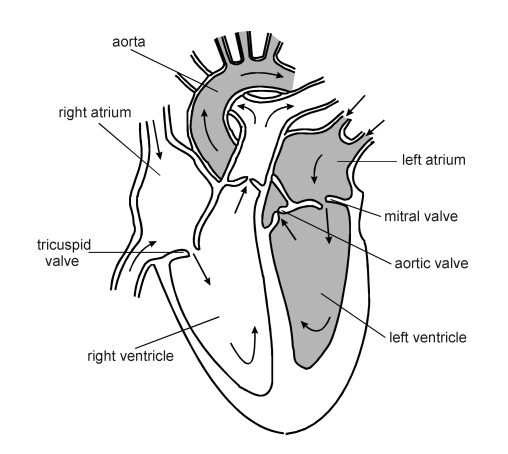
\includegraphics[width=8.5cm]{heart_scheme.eps}
\caption{Изображение аортального клапана и его расположение в сердце}
\end{figure}

Размеры форменных элементов очень малы по сравнению с размерами сосуда
(например, диаметр аорты \(\sim 3 \cdot 10^{-2}\text{м}\), а диаметр
эритроцита \(\sim 6 \cdot 10^{-9}\text{м}\)). Как
показано в \cite{whitmore1968}, отдельно плазма ведет себя как ньютоновская
жидкость. 
Это позволяет нам рассматривать движение крови в крупных 
кровеносных сосудах как течение вязкой, несжимаемой неоднородной 
двухкомпонентной жидкости с переменной вязкостью и плотностью. Стенки 
сосуда и створки клапана будем считать непроницаемыми для жидкости 
поверхностями, которые обладают некоторой жесткостью. Под воздействием 
давления жидкости стенки сосудов и створки клапана могут деформироваться.  

\begin{figure}[t]
\label{fig:aorta_valve_scheme}
\centering
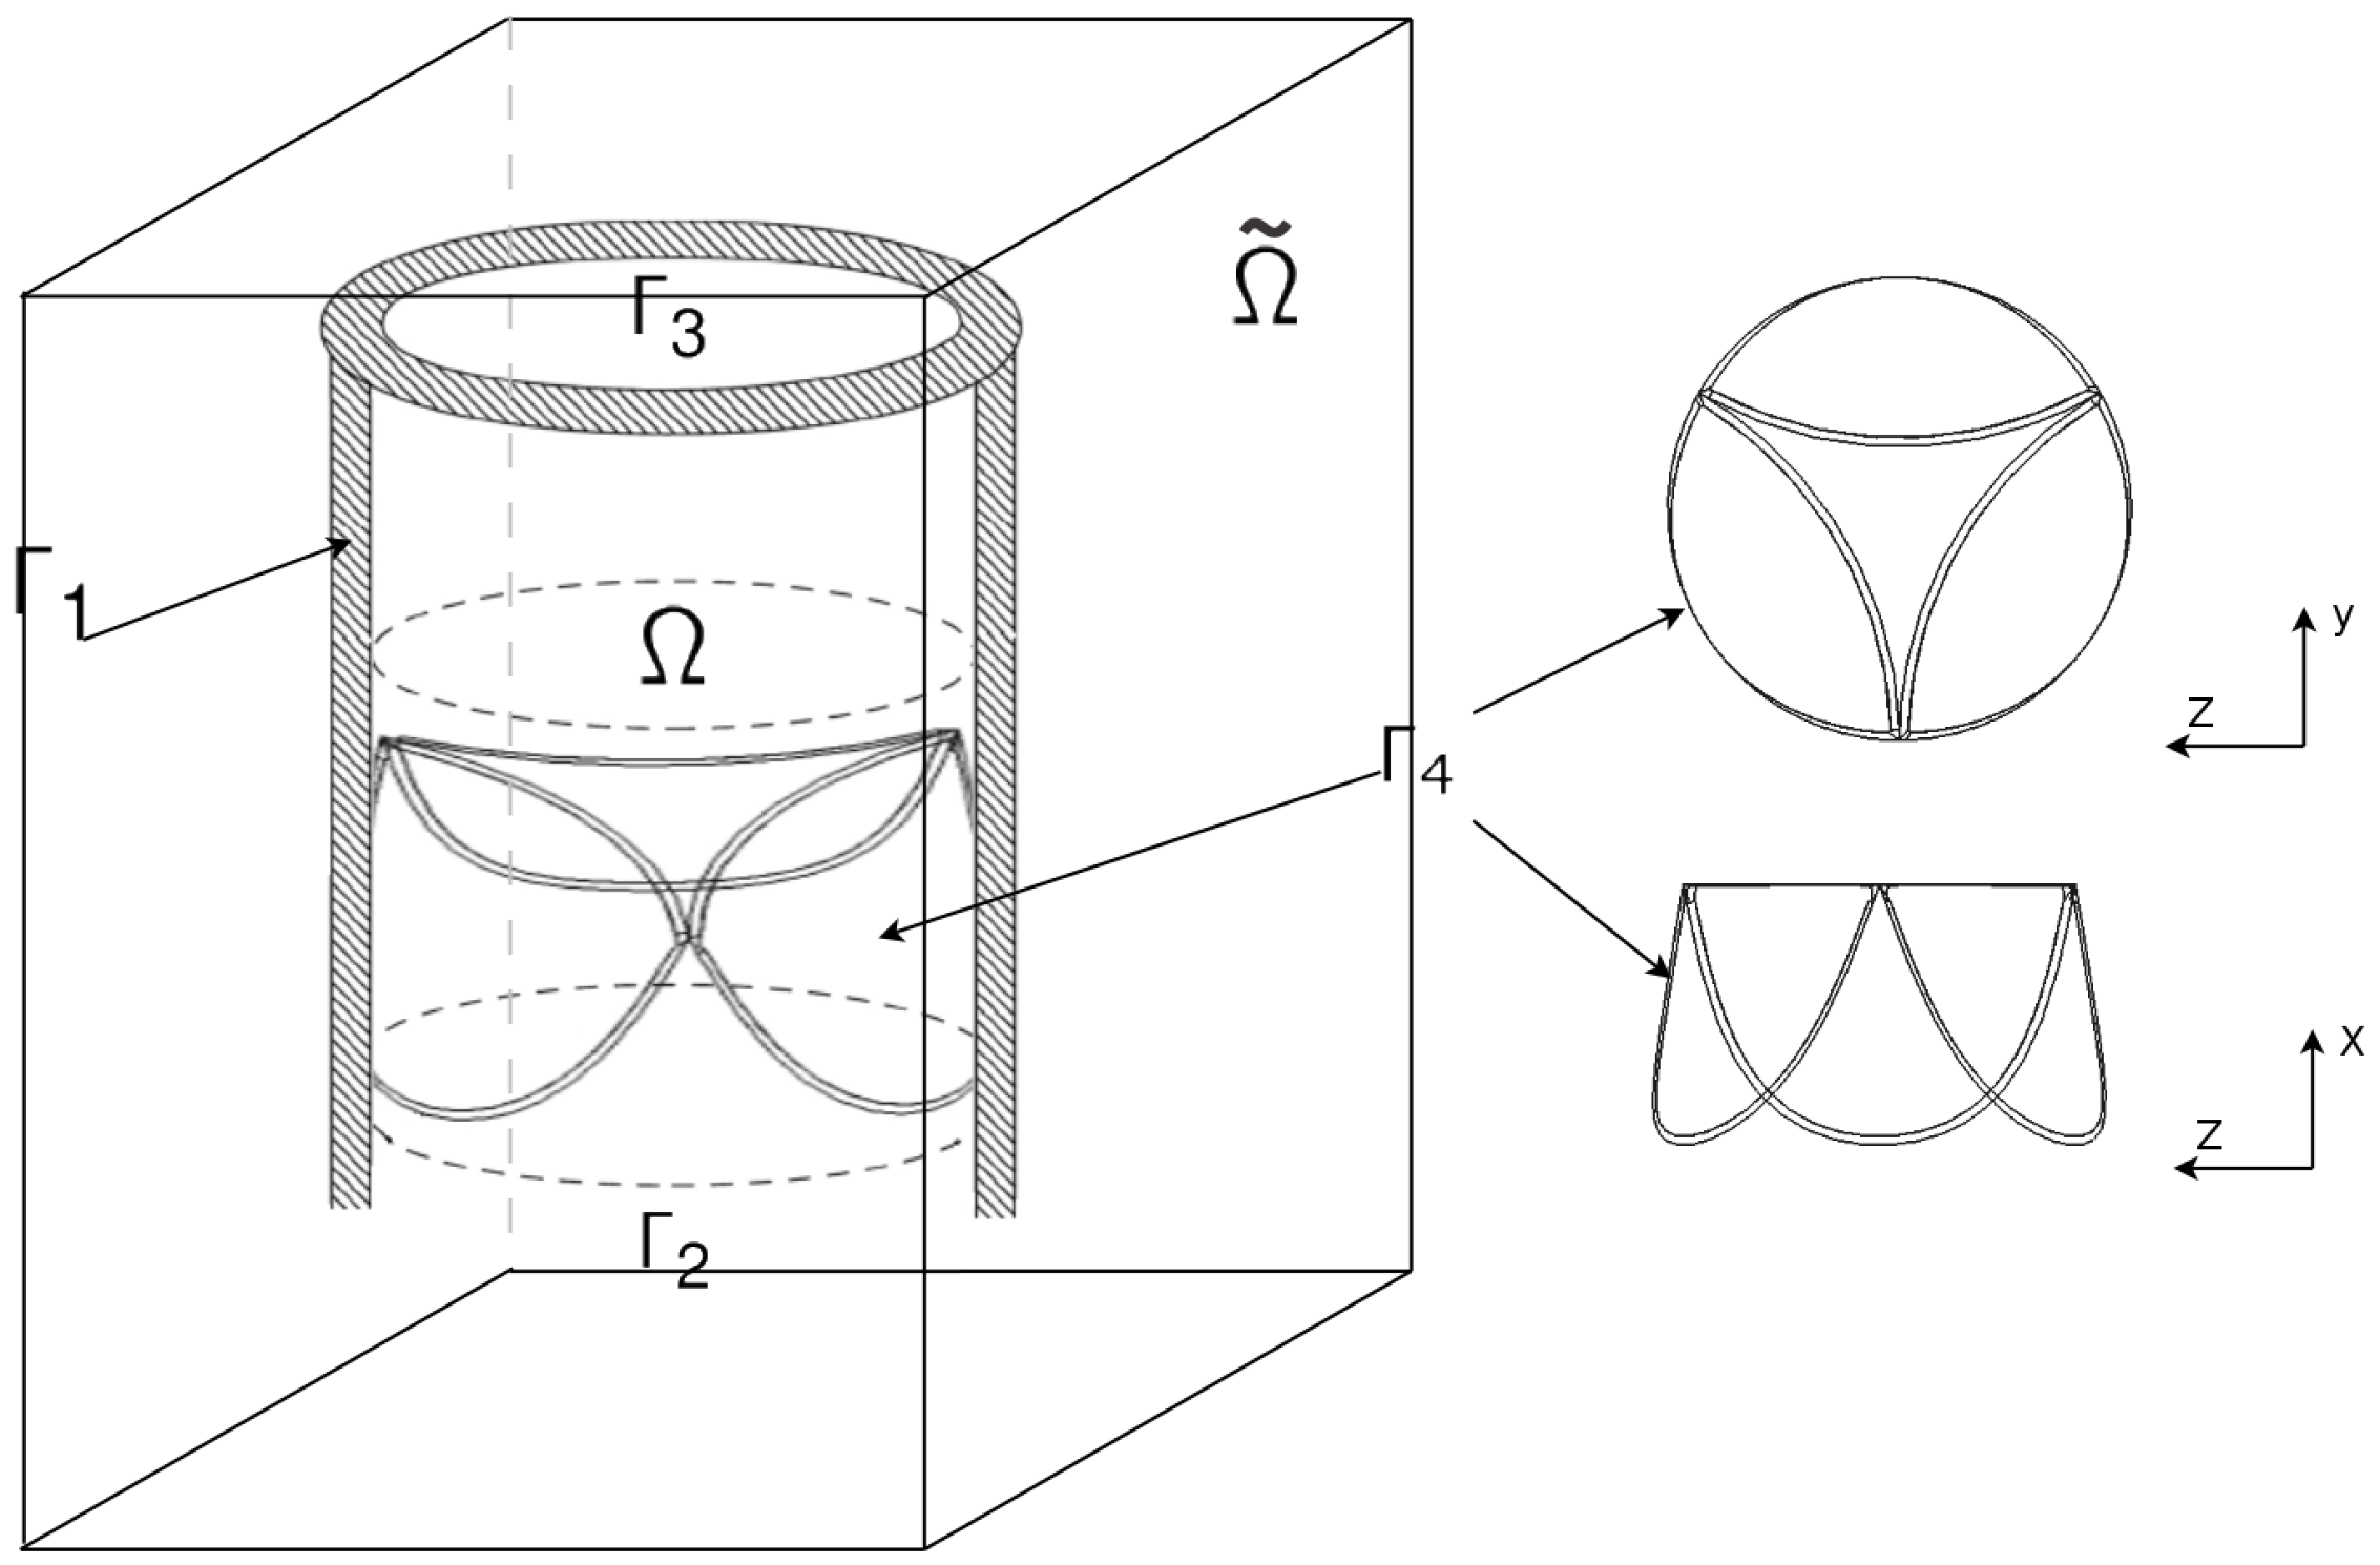
\includegraphics[width=10.5cm]{aorta_valve_scheme_flat_computation.eps}
\caption{Изображение границ расчетной области}
\end{figure}

Так как источником движения крови в сосудах является давление,
создаваемое сокращением сердца, то задачу о движении крови опишем следующей
нестационарной системой дифференциальных уравнений Навье-Стокса
\cite{gummel2013}:

\begin{equation}\frac{\partial \textbf{u}}{\partial t} + (\textbf{u} \cdot \nabla) \textbf{u} = - \frac{1}{\rho} \nabla p + \nabla \sigma + \textbf{f}\label{eq:navier_stokes:motion}\end{equation}

\begin{equation}\frac{\partial \rho}{\partial t} + \nabla \cdot (\rho \textbf{u}) = 0\label{eq:navier_stokes:continuity}\end{equation}

с начальными и краевыми условиями:

\begin{equation}\textbf{u}(\bar{x}, 0) = \textbf{u}_0 \qquad \textbf{u}|_{\Gamma_1, \Gamma_4} = \textbf{u}_b \qquad v,w|_{\Gamma_2, \Gamma3} = 0\label{eq:navier_stokes:velocity_conditions}\end{equation}

\begin{equation}p_{\Gamma_2} = p_{in} \qquad p_{\Gamma_3} = p_{out}\label{eq:navier_stokes:pressure_conditions}\end{equation}

где переменные плотность и вязкость $\rho=\rho(bar{x}, t)$, $\mu=\mu(\bar{x}, t)$
определяются следующим образом:

\begin{equation}\mu = c (\mu_2 - \mu_1) + \mu_1\label{eq:viscosity}\end{equation}

\begin{equation}\rho = c (\rho_2 - \rho_1) + \rho_1\label{eq:density}\end{equation}

Здесь $\mu_1, \mu_2, \rho_1, \rho_2$ - вязкости и плотности несущей жидкости (плазмы) и примеси (форменных элементов)
соответственно, $c$ - концентрация примеси,
\(\bar{x}=(x,y,z) \in \Omega\), \(\textbf{u}=(u,v,w)\) - вектор
скорости с компонентами \(u(x, y, z), v(x, y, z), w(x, y, z)\),
\(\textbf{u}_b\) - скорость движения створок клапана под
воздействием деформации, \(\rho=\rho(\bar{x}, t)\) - плотность,
\(p=p(\bar{x}, t)\) - давление,
\(\sigma = \mu (\nabla \textbf{u} + (\nabla \textbf{u})^T)\) - вязкий тензор
напряжений, \(\mu = \mu(\bar{x}, t)\) - вязкость жидкости,
\(\textbf{f} = \textbf{f}(\bar{x}, t)\) - вектор массовых сил. Область
\(\Omega\) представляет собой сосуд с границами
\(\Gamma = \Gamma_1 \cup \Gamma_2 \cup \Gamma_3 \cup \Gamma_4\), где
\(\Gamma_1\) - стенки кровеносного сосуда, \(\Gamma_2\) and \(\Gamma_3\)
- границы, на которых происходит втекания/вытекания, \(\Gamma_4\) - створок клапана (см рис.
\ref{fig:aorta_valve_scheme}).

Концентрация определяется как решение уравнения переноса:

\begin{equation}\frac{\partial c}{\partial t} + \textbf{u} \cdot \nabla c = 0\label{eq:convection}\end{equation}

с начальными условиями:

\begin{equation}c(\bar{x}, 0) = c_0(\bar{x}), \bar{x} \in \Omega\label{eq:convection:conditions}\end{equation}

с краевыми условиями для области втекания:

\begin{equation}c(\bar{x}, t)|_{\Gamma_2} = c_s(\bar{x}, t)\label{eq:convection:conditions}\end{equation}

Отсутствие задания одной компоненты вектора скорости $u(x, y, z, t)$ на участках
втекания-вытекания является одной из проблем при численном решении задач
подобного типа. Она решается с помощью использования исходных уравнений
(\ref{eq:navier_stokes:motion}) - (\ref{eq:navier_stokes:continuity}) на
границах \(\Gamma_2\) и \(\Gamma_3\) для вычисления недостающих
компонент вектора скорости (подробнее см. \cite{gummel2013}, \cite{dolgov2015vestnik}).

Для того, чтобы иметь возможность моделировать движение тонких гибких клапанов,
необходимо добавить силы, возникающие при деформации створок клапана и
стремящиеся вернуть их в равновесное состояние. 

Для описания сил, возникающих при деформации клапана, воспользуемся
следующей формулой (см.\cite{peskin2002}, \cite{griffith2012}):

\begin{equation}F = \frac{\partial}{\partial s} T \bm{\tau} + \frac{\partial^2}{\partial s^2} \left( k \cdot \left(\frac{\partial^2 X^0}{\partial s^2} - \frac{\partial^2 X}{\partial s^2} \right) \right)\label{eq:resulting_force}\end{equation}
где $\bar{q}=(q,r,s) \in \Gamma$, $X = X(\bar{q}, t)$ - функция,
описывающая поверхность створок клапана в момент времени $t$, 
$X^0 = X(\bar{q}, 0)$, координаты $q,r,s$ выбраны так, чтобы поверхность
$X$ была представлена набором параметрических линий $s \to X(q^*,r^*,s)$,
$T$ - напряжение, возникающее вдоль линии $s \to X(q^*,r^*,s)$,
$\bm{\tau}$ - единичный вектор, касательный к поверхности клапана,
\(k = E \cdot I\), \(E\) - модуль упругости, \(I\) - момент инерции
поперечного сечения.

Как показано в \cite{peskin2002}, для того, чтобы описать взаимодействие потока
жидкости и клапана, необходимо ввести в рассмотрение параллелепипед $\tilde{\Omega}$, содержащий внутри себя \(\Omega\). Тогда движение гибкой границы в жидкости определяется из следующего уравнения:

\begin{equation}\frac{\partial X}{\partial t}(\bar{q}, t) = \int_{\Omega} \textbf{u}(\bar{x}, t) \cdot \delta (x - X(\bar{q}, t))\; d\bar{x}\label{eq:interaction:velocity}\end{equation}

и правая часть системы \ref{eq:navier_stokes:motion} задается следующим образом:

\begin{equation}\textbf{f}(\bar{x}, t) = \int_{\Gamma} \textbf{F}(\bar{q}, t) \cdot \delta (x - X(\bar{q}, t))\; d\bar{q}\label{eq:interaction:force}\end{equation}

где \(\delta\) - дельта функция Дирака, \(F\) - сила
деформации. 

Таким образом, уравнения \ref{eq:navier_stokes:motion} - \ref{eq:interaction:force} описывают взаимодействие крови как вязкой
неоднородной несжимаемой жидкости с переменной вязкостью и плотностью с искусственным сердечным клапаном. В этой
модели состояние жидкости и форма поверхностей
\(\Gamma_1 \cup \Gamma_4\) определяются независимо друг от друга, а
влияние створок клапана на течение отражено с помощью соотношения
(\ref{eq:interaction:force}) между вектором массовых сил
\(\textbf{f}(\bar{x}, t)\) уравнения (\ref{eq:navier_stokes:motion}) и
силой сопротивления деформации \(F=F(\bar{q}, t)\) из уравнения
(\ref{eq:resulting_force}).

\section{Метод решения}

В данной работе для определения движения створок клапана мы будем использовать
метод погруженной границы \cite{peskin2002}. В соответствии с этим методом,
будем рассчитывать течение жидкости в параллелепипеде \(\tilde{\Omega}\),
который включает в себя \(\Omega\) (см. рис \ref{fig:aorta_valve_scheme}). На границах \(\tilde{\Omega}\) задано
условие прилипания. Для расчета течения жидкости будем использовать
прямоугольную равномерную разнесенную сетку \(\tilde{\Omega_h}\) с
шагами \(h_{xi}, h_{yj}, h_{zk}\) и шахматным расположением узлов, где
давление, дивергенция скорости и концентрация определяются в центре
ячейки, а компоненты вектора скорости и внешних сил -- на границах. 

Алгоритм решения состоит из нескольких шагов: на сетке \(\tilde{\Omega_h}\)
решаем задачу
(\ref{eq:navier_stokes:motion})-(\ref{eq:navier_stokes:pressure_conditions});
затем решаем уравнение конвекции (\ref{eq:convection}) т.е. определяем
концентрацию примеси в области решения и пересчитываем значение
плотности и вязкости. После этого используем формулы
(\ref{eq:resulting_force}) и (\ref{eq:interaction:velocity}),
(\ref{eq:interaction:force}) для определения положения створок клапана и их 
формы

Поставленная дифференциальная задача (\ref{eq:navier_stokes:motion}) --
(\ref{eq:density}) решается методом конечных разностей. Для решения
(\ref{eq:navier_stokes:motion}) --
(\ref{eq:navier_stokes:pressure_conditions}) будем использовать схемы
расщепления по физическим факторам \cite{belotserkovsky1984}:

\begin{equation}\frac{u^* - u^n}{\triangle t} = - (u^n \cdot \nabla) u^* - \frac{1}{\rho}
\nabla \sigma + f^n\label{eq:splitting:intermediate_velocity}\end{equation}

\begin{equation}\rho \triangle p^{n+1} - \nabla \rho \cdot p^{n+1} = \frac{\rho^2 \nabla
u^*}{\triangle t} \label{eq:splitting:poisson}\end{equation}

\begin{equation}\frac{u^{n+1} - u^*}{\triangle t} = - \frac{1}{\rho} \triangle p^{n+1} \label{eq:splitting:velocity}\end{equation}

Численная реализация схемы состоит из 3-х этапов. Сначала по известным
значениям скорости с предыдущего временного слоя находится промежуточное
поле \(u^*\). Для этого уравнение
(\ref{eq:splitting:intermediate_velocity}) решается методом
стабилизирующей поправки \cite{yanenko1967}. Затем, путем численного решения
(\ref{eq:splitting:poisson}) с использованием метода бисопряженных
градиентов, определяется новое поле давления. И на последнем этапе
восстанавливается окончательное поле вектора скорости по явным формулам
(\ref{eq:splitting:velocity}).

После нахождения параметров течения жидкости необходимо вычислить новые
значения плотности и вязкости. Для этого, используя полученные значения
компонент скорости, делается шаг по времени для уравнения конвекции
(\ref{eq:convection}), и производится пересчет значений плотности и
вязкости по формулам (\ref{eq:viscosity}), (\ref{eq:density}).

Далее нам необходимо определять деформацию стенок сосуда и створок
клапана под воздействием жидкости, а также распределение массовых сил $\textbf{f(q,r,s,t)}$ в
уравнении движения жидкости исходя из возникшей деформации. Используя
уравнения (\ref{eq:interaction:velocity}) --
(\ref{eq:interaction:force}), которые численно интегрируются с помощью
обобщенной квадратурной формулы трапеций, и уравнение (\ref{eq:resulting_force}),
мы можем рассчитать деформацию, которой подвергаются стенки сосуда и
клапан при данном давлении жидкости и возникающую силу сопротивления
\(F(q,r,s,t)\). После этого пересчитываем массовые силы $\textbf{f(q,r,s,t)}$ и переходим на следующий шаг по времени.

\section{Результаты}

В этом пункте приведем некоторые результаты методических расчётов работы
искусственных сердечных клапанов. Расчеты проводились для случаев постоянной и
переменной плотности и вязкости в безразмерных величинах.

Все численные эксперименты проводились для двух клапанов: идеальный клапан
упрощенной формы и клапан, полученный сканированием реального
биопротеза “Юнилайн” (см. рис. \ref{fig:uniline}) \cite{klyshnikov2013}.

\begin{figure}[t]
\label{fig:uniline}
\centering
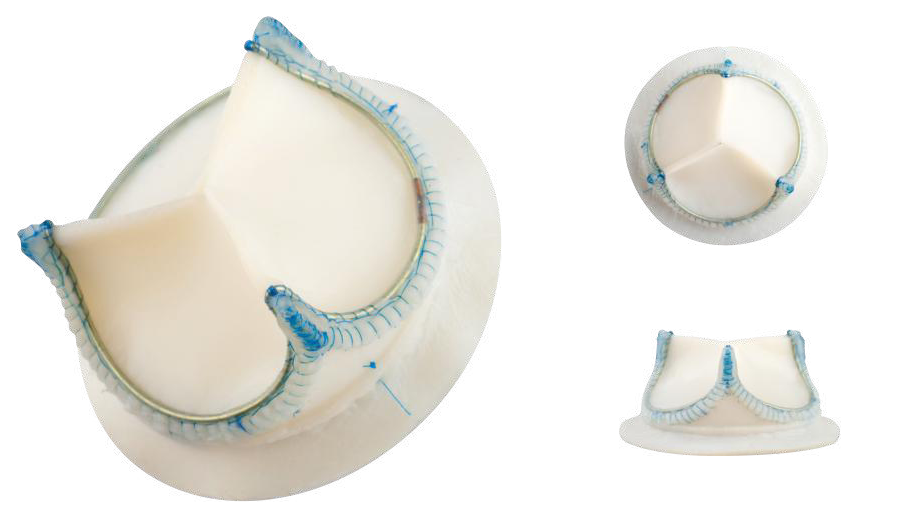
\includegraphics[width=8.5cm]{uniline_real_no_alpha.eps}
\caption{Искусственный клапан "Юнилайн"}
\end{figure}

В качестве сосуда, в котором расположен клапан, для всех расчетов используется круговой цилиндр (см. рис. \ref{fig:aorta_valve_scheme})
с длинной \(l=1\), радиусом \(r=0.11\) и жесткостью стенок
\(k=1 \cdot 10^{3}\). Для створок клапана заданы коэффициенты
сопротивления растяжению \(k_s = 5 \cdot 10^{3}\) и скручиванию
\(k_b = 2 \cdot 10^{3}\). Перепад давления \(p_{in} - p_{out}\)
периодически меняется от 0 до 6 с параболической зависимостью от времени на каждом периоде.
Область \(\tilde{\Omega}\) имеет размеры \(10 \times 0.5 \times 0.5\). Далее приведены результаты
расчетов для пространственной сетки $\tilde{\Omega_h}$ с шагом по времени $\triangle t = 0.01$
шаги по пространственной сетке
\(\tilde{\Omega_h}\) \(h_x = h_y = h_z = 0.01\), шаг по времени
\(\triangle t = 0.01\).

На рис. \ref{fig:valve_motion} показано движение створок клапана и течение
жидкости через него при увеличении и уменьшении перепада давления.

\begin{figure}[!htbp]
\centering
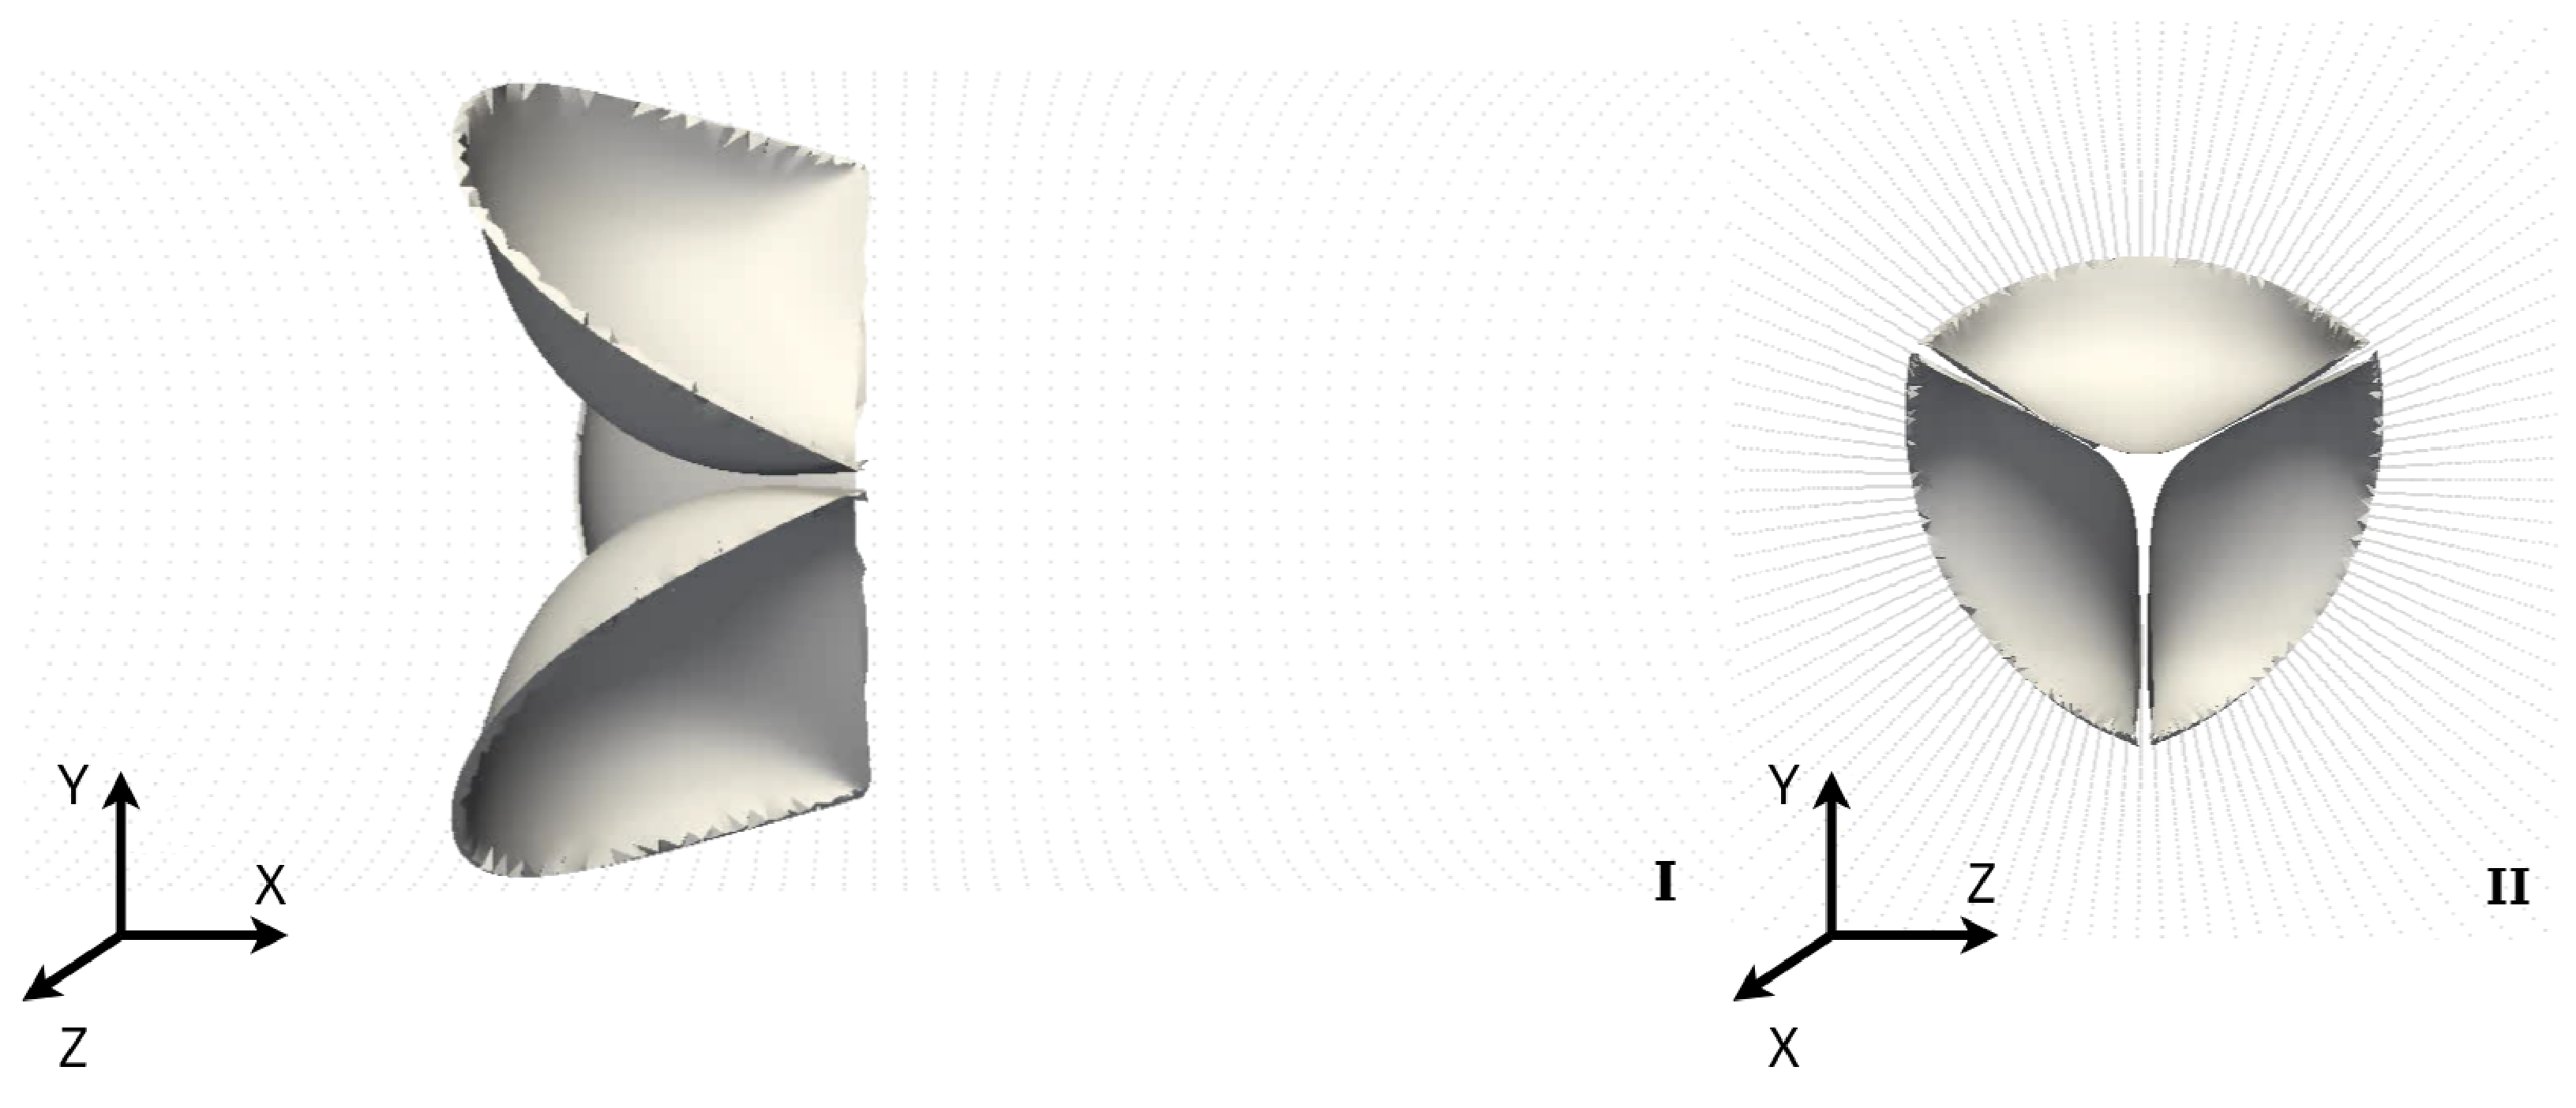
\includegraphics[width=10.5cm]{valve_delaunay_with_markers1_axes.eps}

a

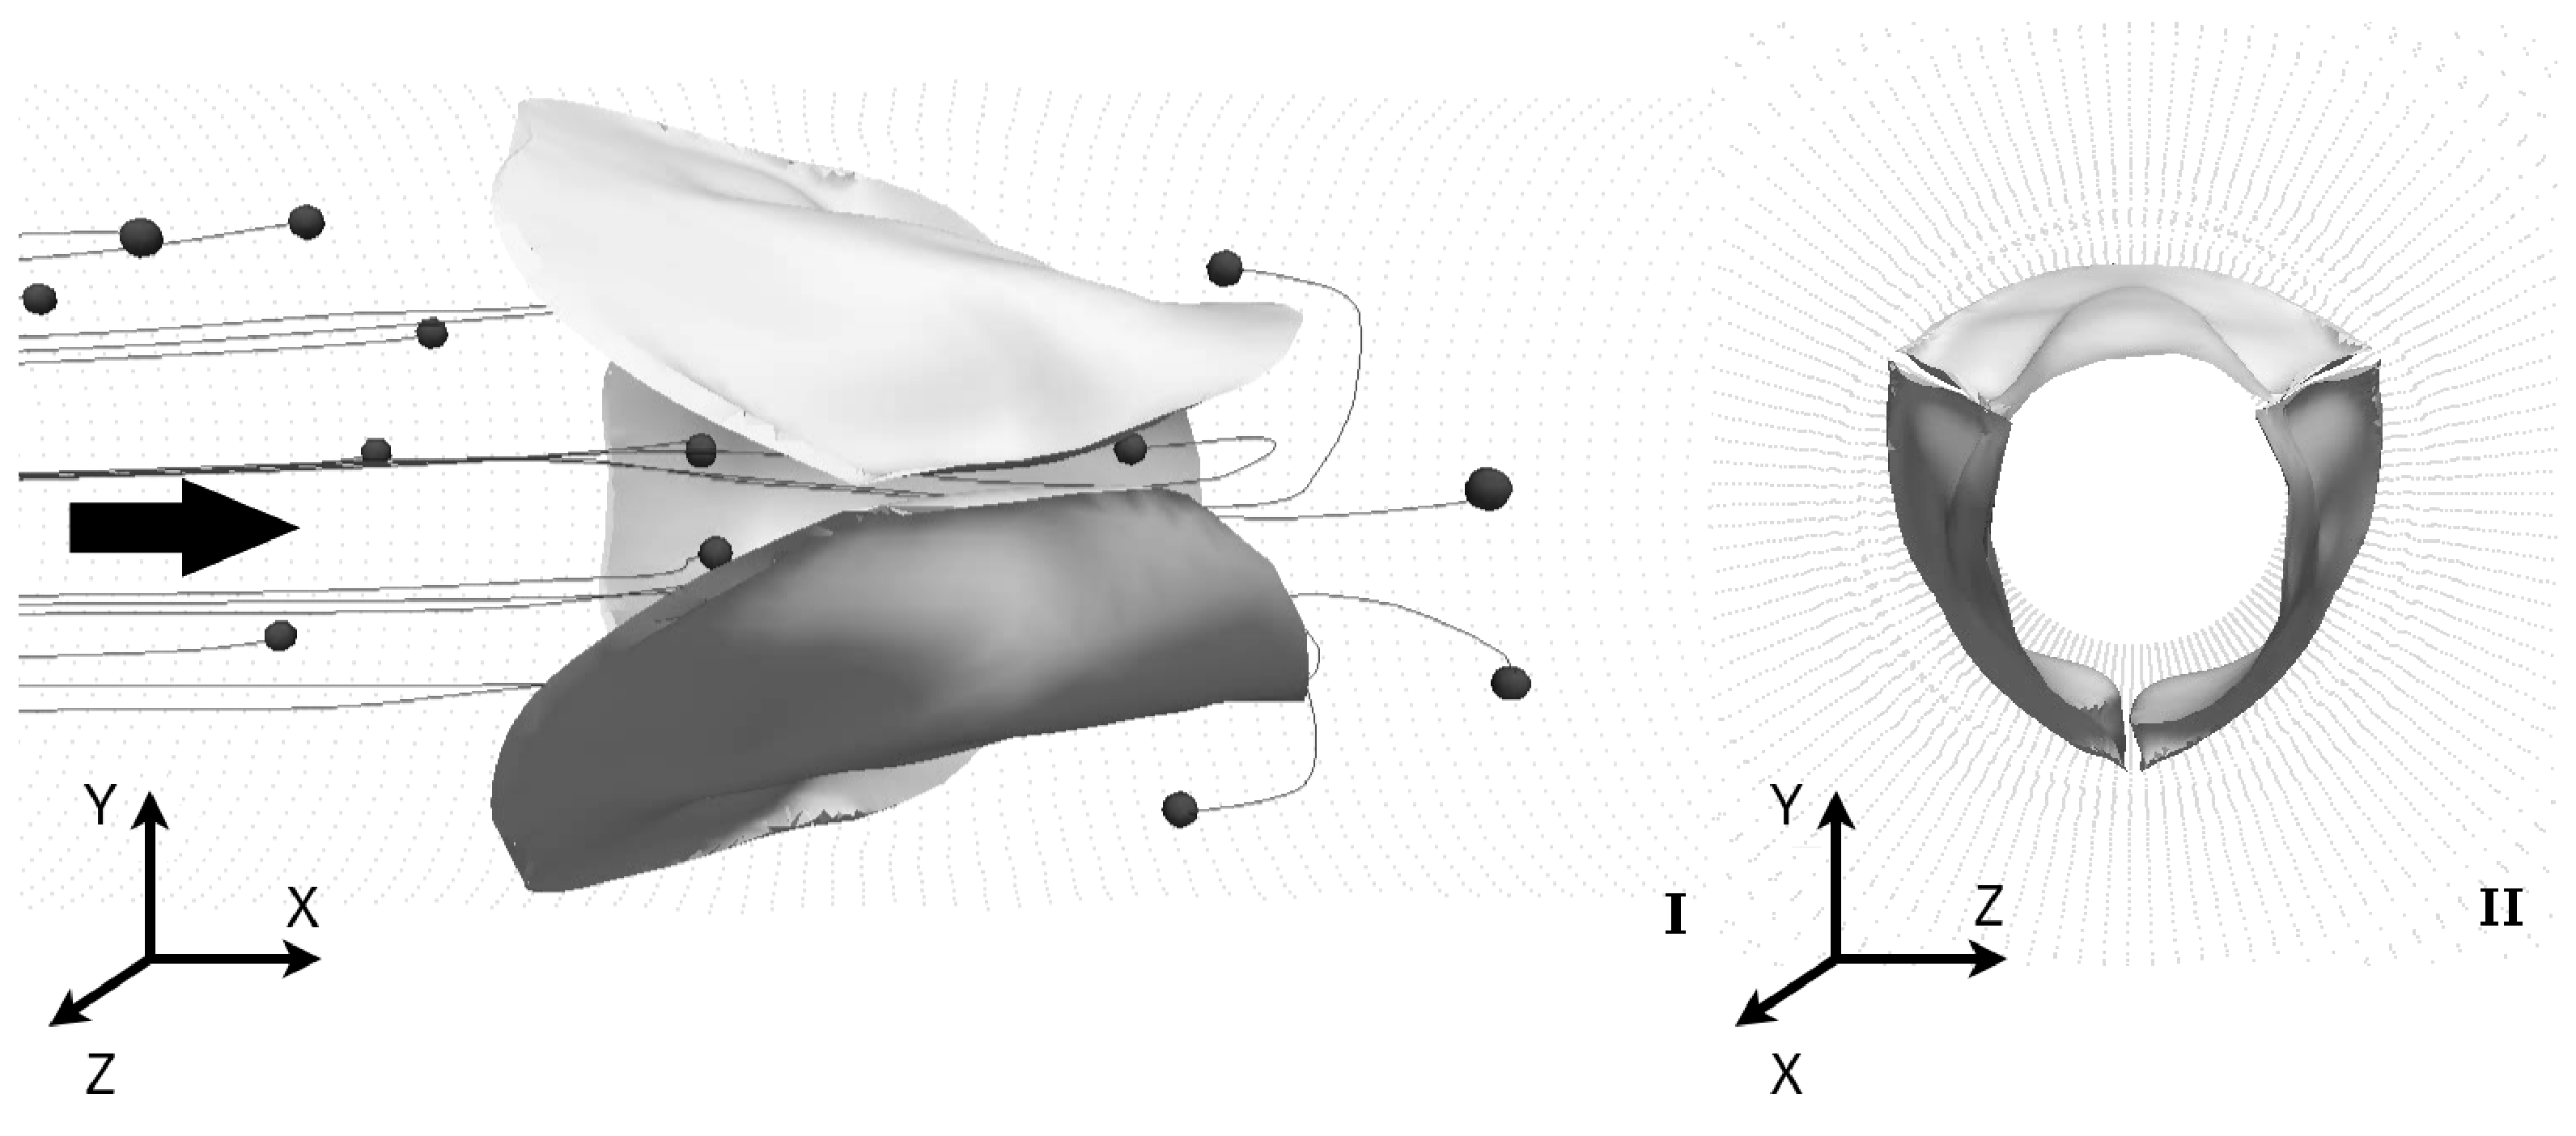
\includegraphics[width=10.5cm]{valve_delaunay_with_markers2_axes.eps}

b

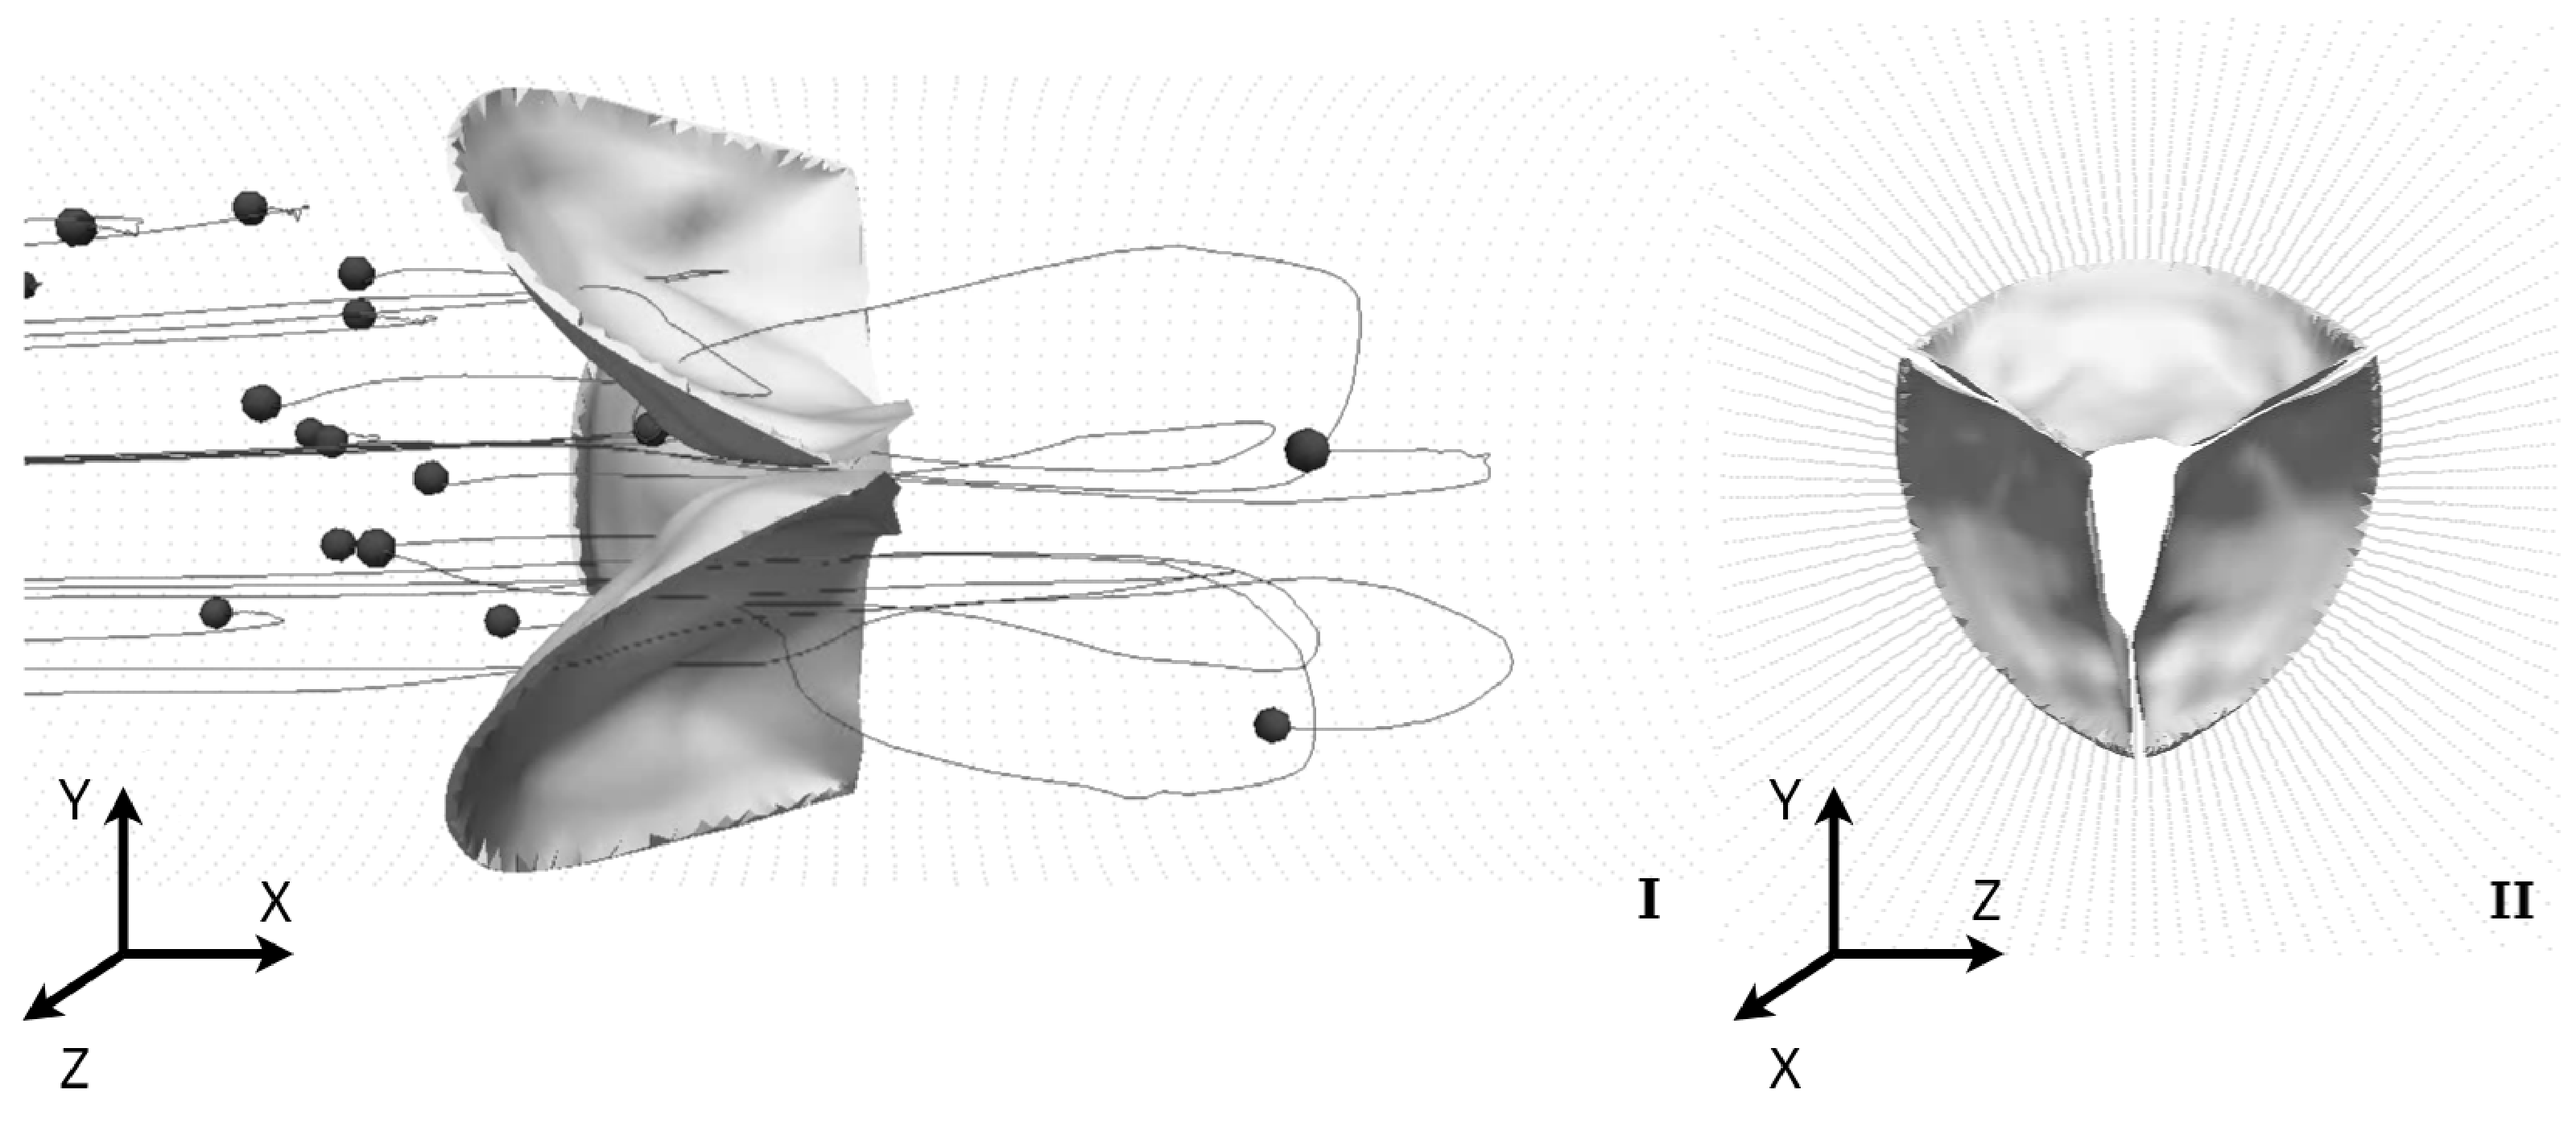
\includegraphics[width=10.5cm]{valve_delaunay_with_markers3_axes.eps}

c

\caption{Динамика створок клапана и треки некоторых частиц. Направление тока
    указано стрелкой. Показан вид сбоку (I) и вид спереди (II) a) $t=0$, b)
    $t=0.7$, c) $t=1.5$}
\label{fig:valve_motion}
\end{figure}

Как можно увидеть из рис. \ref{fig:valve_motion}, створки клапана раскрываются
при изменении разности давлений, а затем возвращаются в исходное положение при
выравнивании давлений.

На рис. \ref{fig:concentration_dynamics} показано изменение концентрации
форменных элементов при прохождении потока жидкости через клапан. Изначально
равномерное распределение форменных элементов со временем нарушается движением
створок клапана.

\begin{figure}[!htbp]
\centering
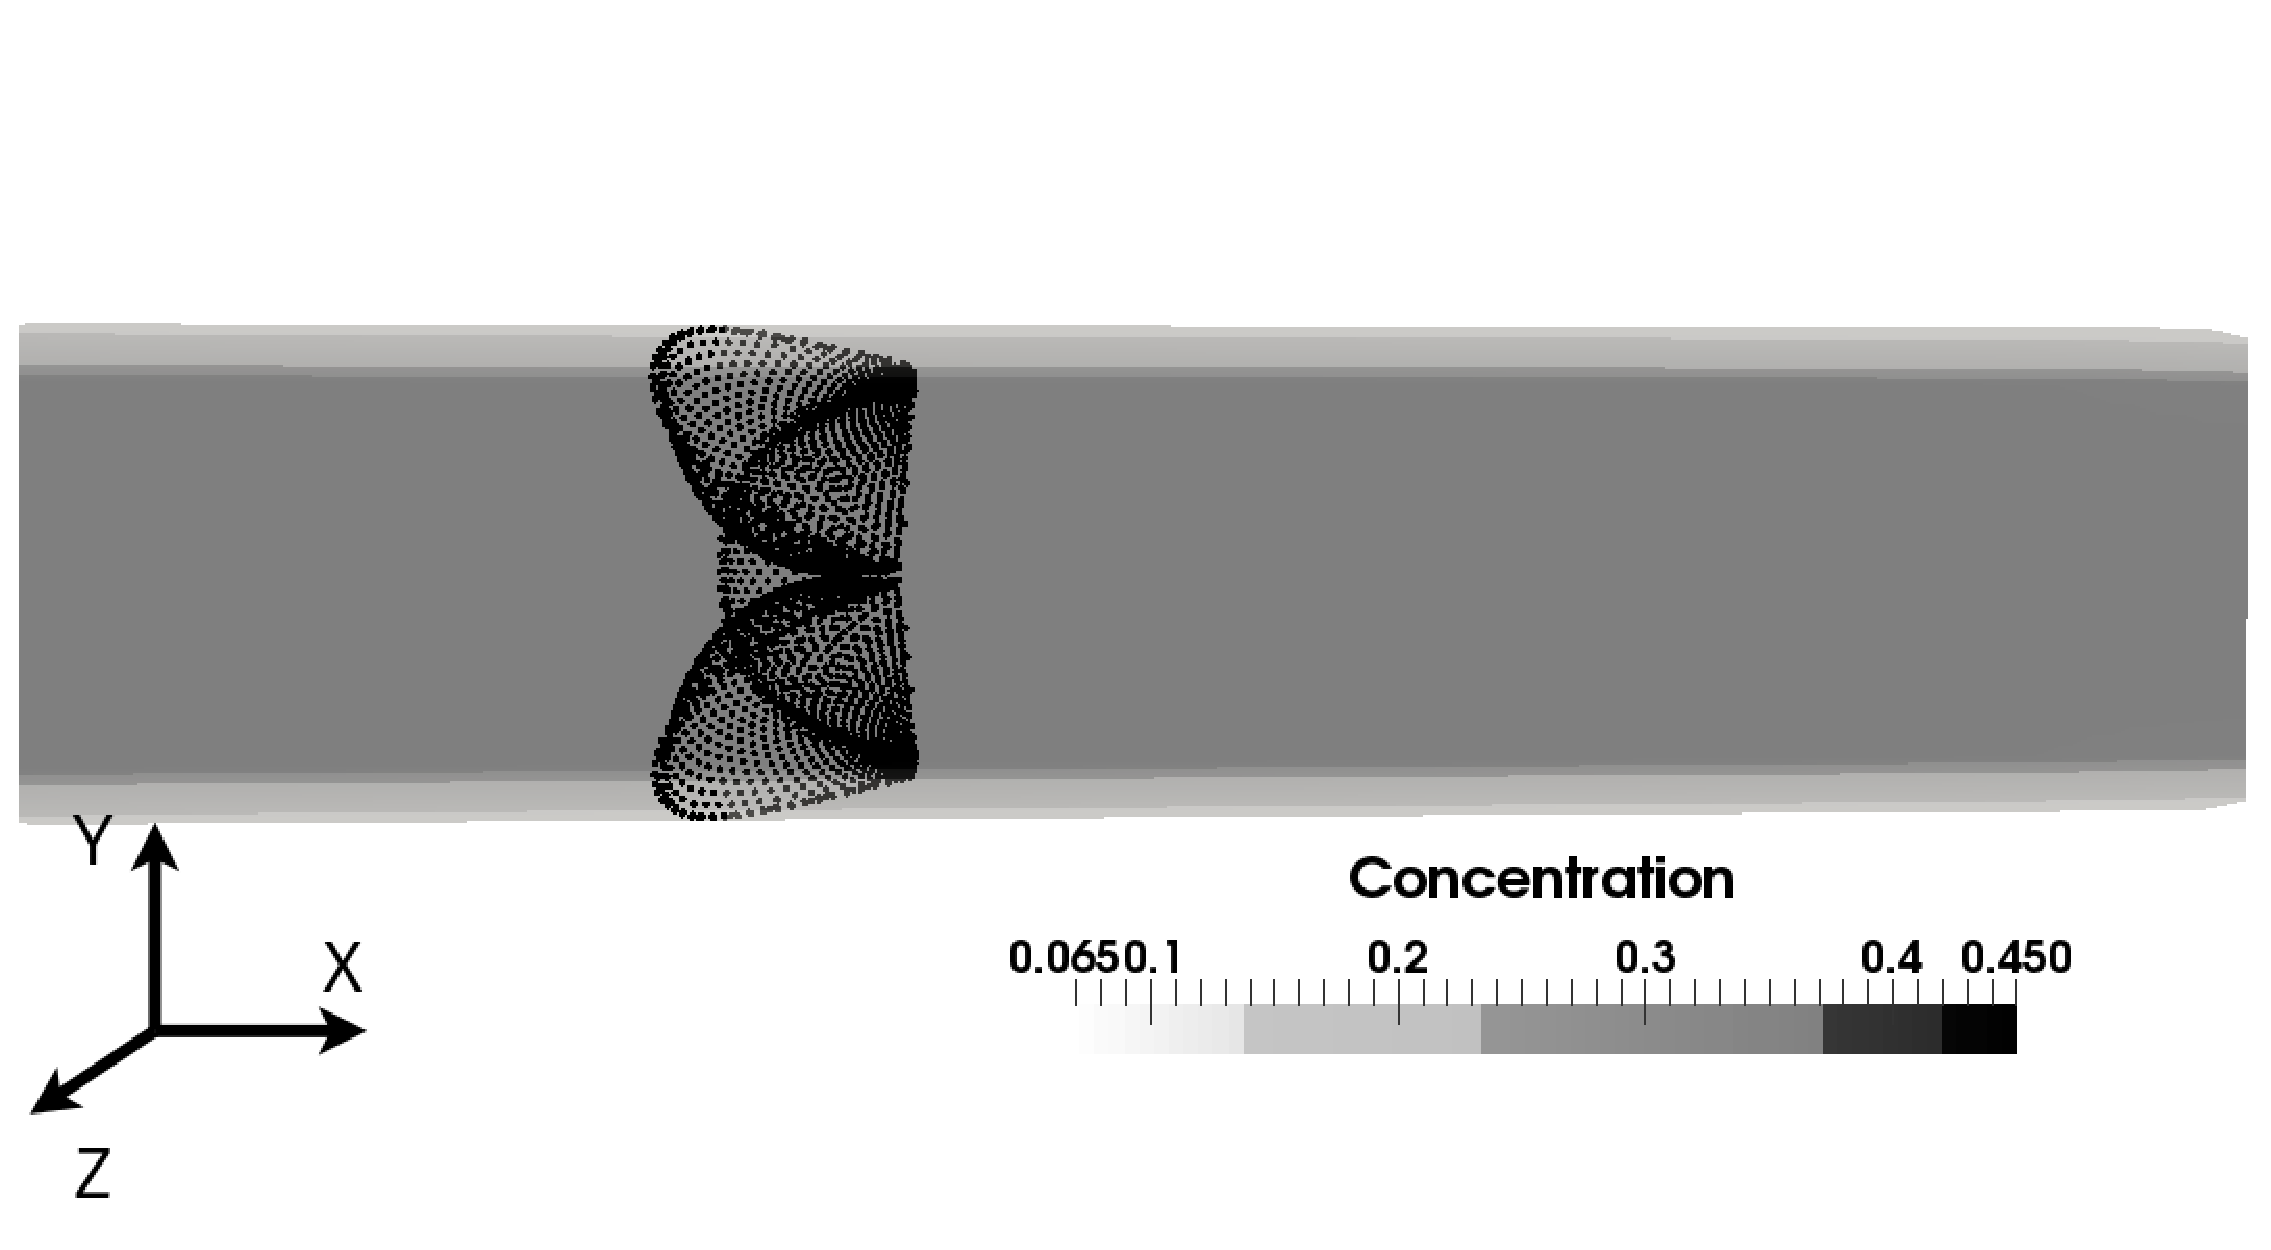
\includegraphics[width=10.5cm]{concentration_1_axes.eps}

a

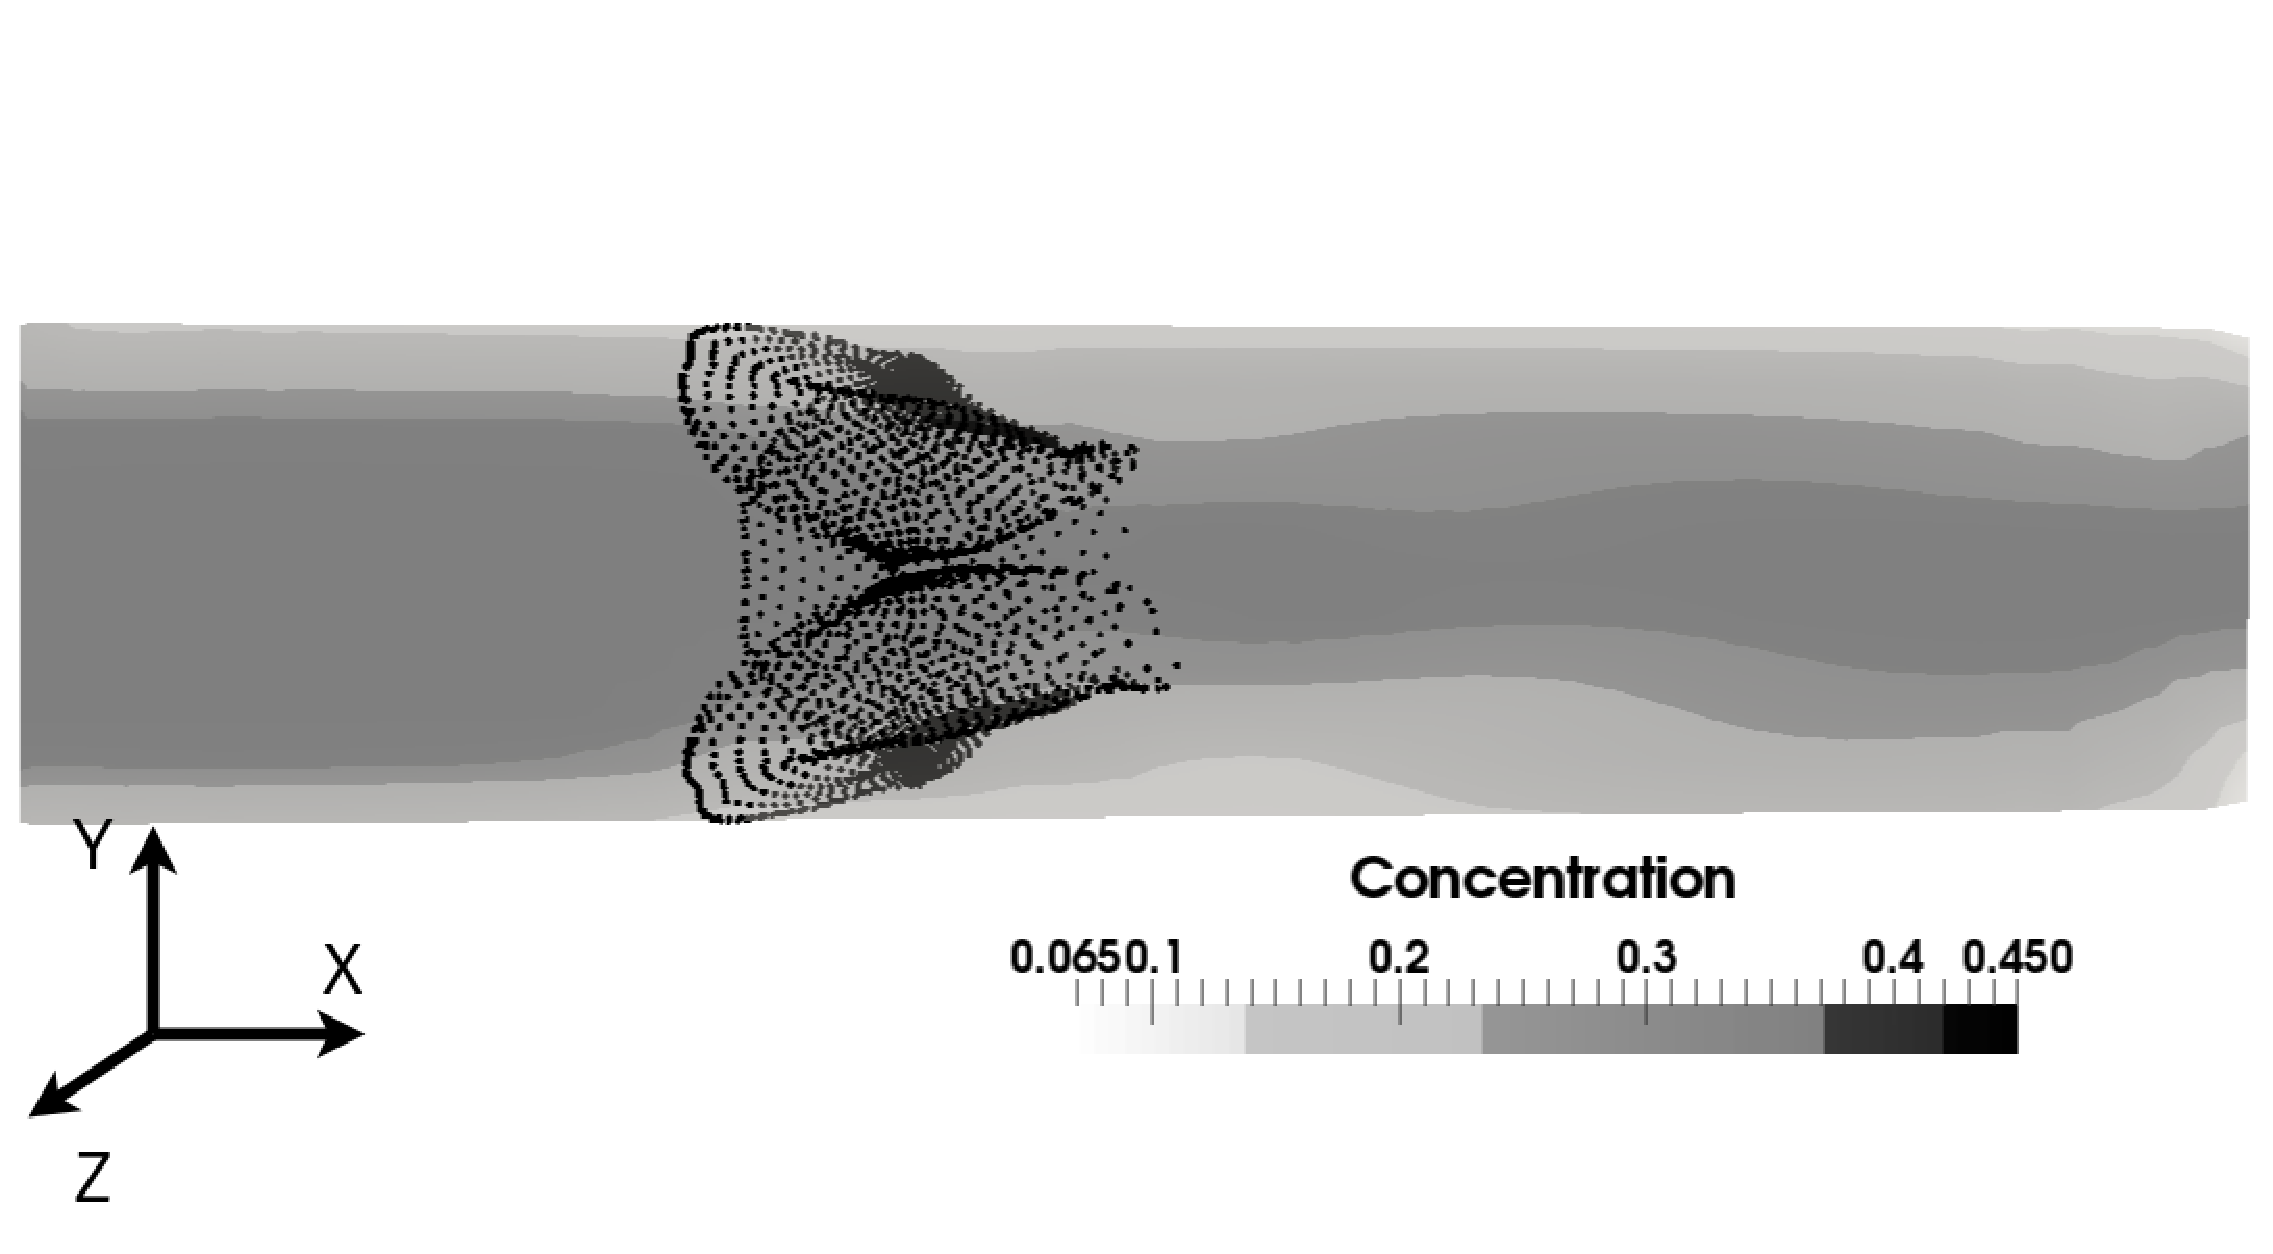
\includegraphics[width=10.5cm]{concentration_2_axes.eps}

b

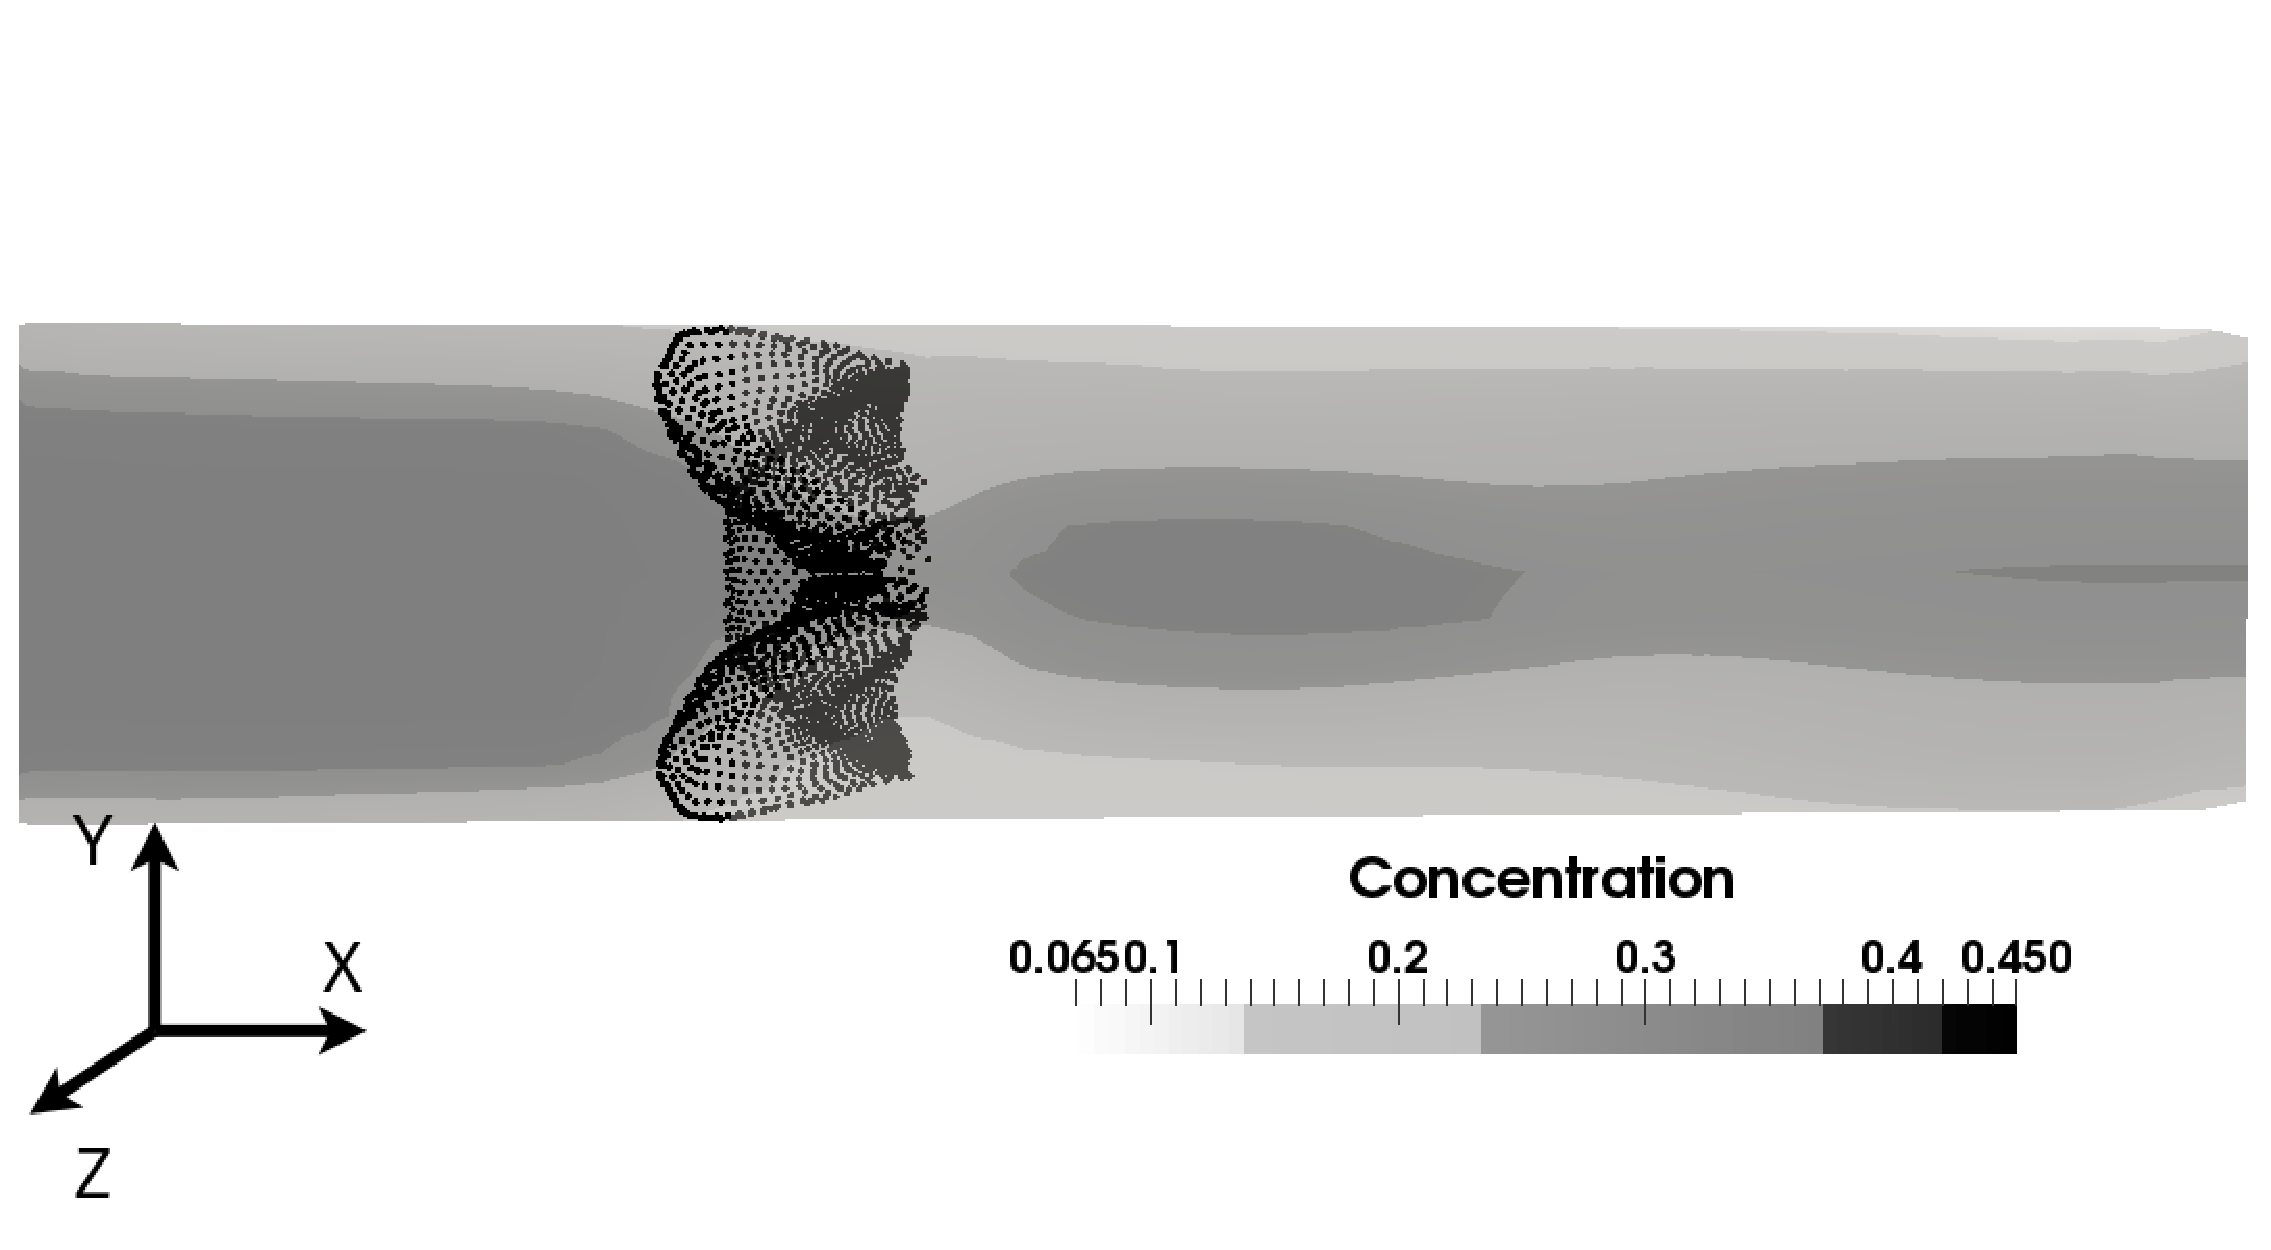
\includegraphics[width=10.5cm]{concentration_3_axes.eps}

c

\caption{Движение створок клапана в сосуде с переменной вязкостью и плотностью.
    На входе задается постоянный приток примеси $c_s|_{\Gamma_2} = 0.45$,
    концентрация примеси в начальный момент времени $c_0=0.45$, $\rho_1=1,
    \rho_2=1.2, \nu_1=1 \cdot 10^{-2}, \nu_2=1.2 \cdot 10^{-2}$; a) $t=0$, b)
    $t=3$, c) $t=6$}
\label{fig:concentration_dynamics}
\end{figure}

На рис. \ref{fig:flow_rate} показан график расхода жидкости внутри клапана в
зависимости от времени для первых трех циклов работы. Каждому пульсу
соответствует резкое повышение расхода, а колебания створок клапана при
закрытии отражаются  в осцилляции на графике. 

\begin{figure}[t]
\centering
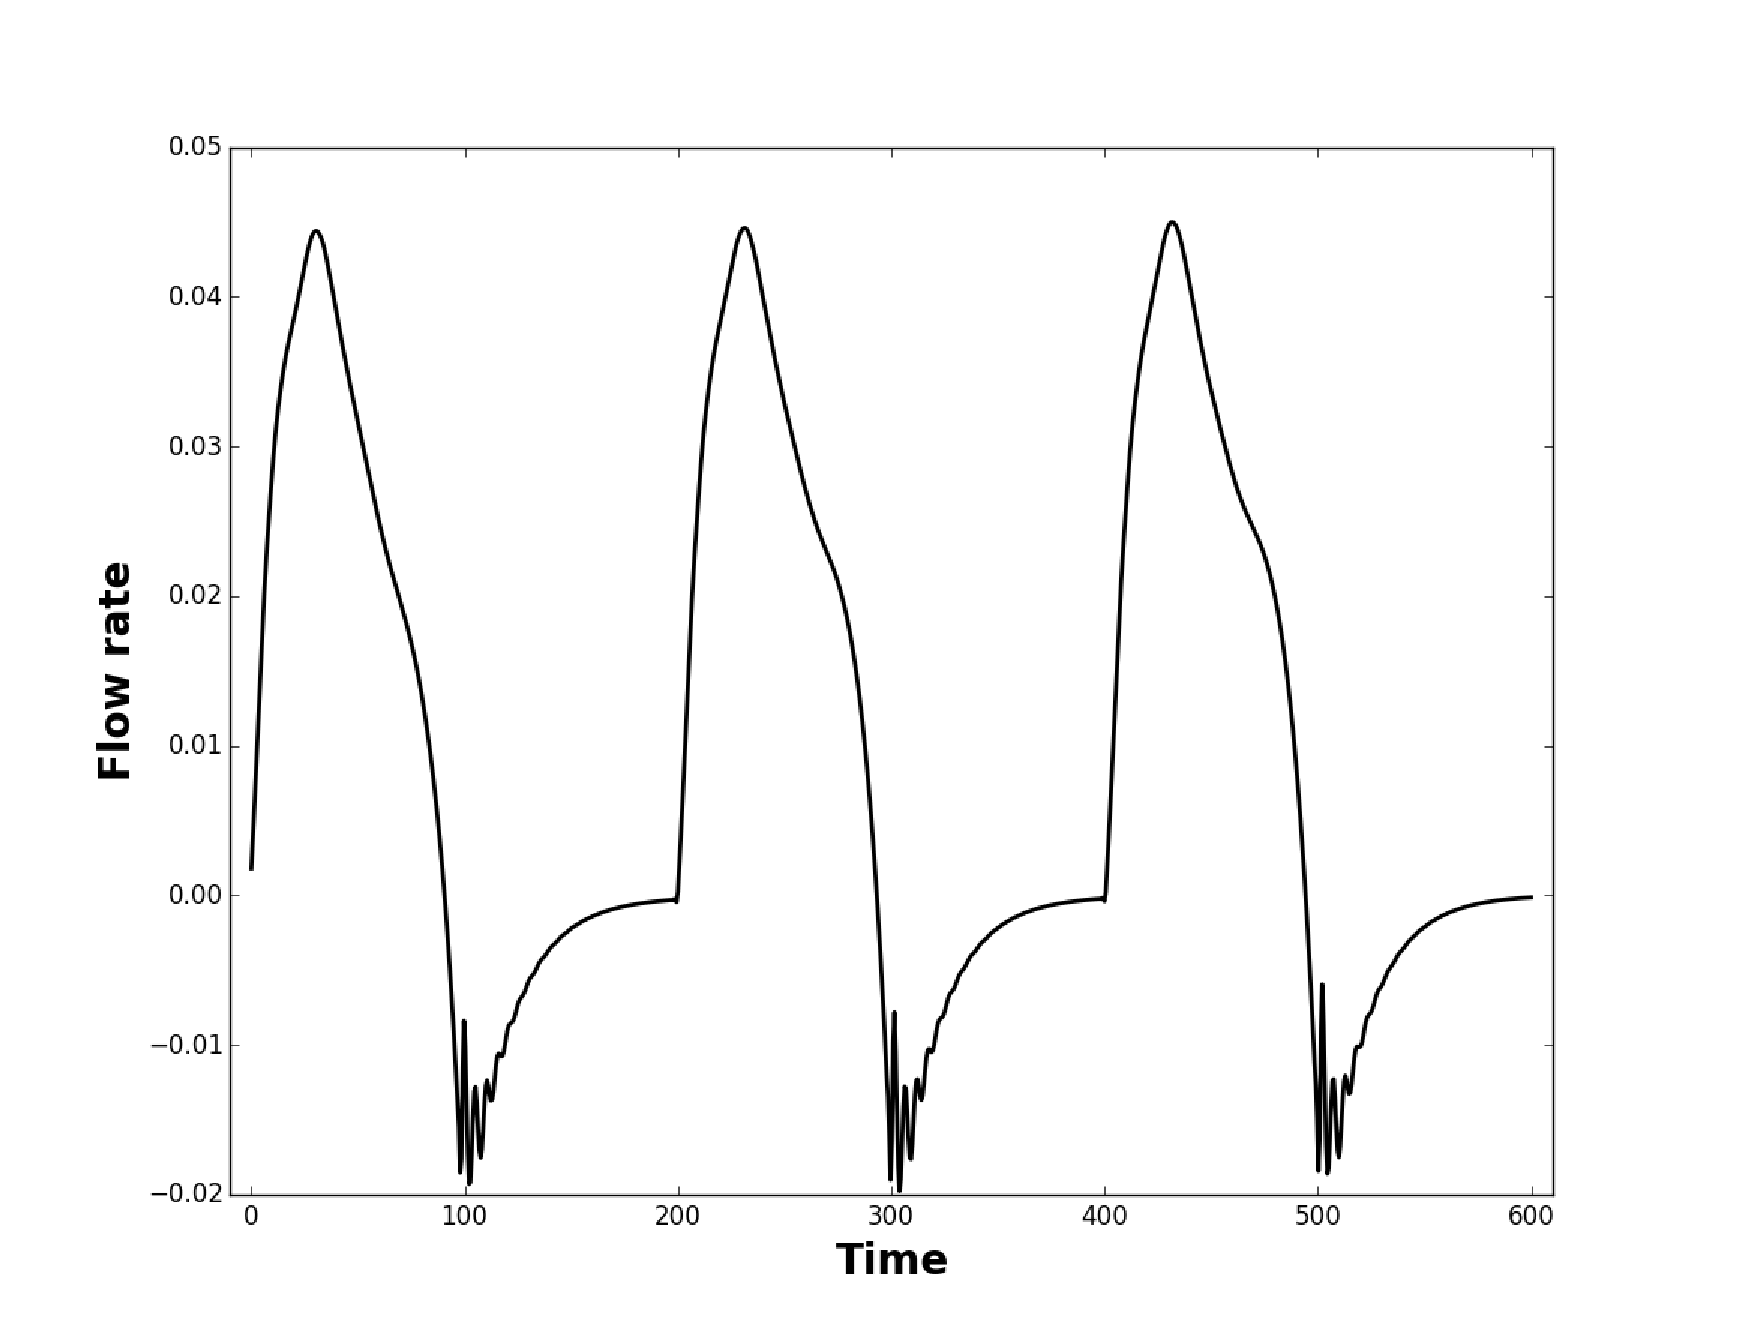
\includegraphics[width=10.5cm]{flow_rate_separate.eps}
\caption{График расхода жидкости в зависимости от времени}
\label{fig:flow_rate}
\end{figure}

На рис. \ref{fig:ideal_valve_stress} показана динамика движения одной
створки идеального трехстворчатого клапана под воздействием жидкости с
переменной вязкостью и плотностью
\(\rho_1=1, \rho_2=2, \mu_1=1\ cdot 10^{-2}, \mu_2=2 \cdot 10^{-2}\), а также распределение
напряжения $F(q,r,s,t)$ по поверхности (см. уравнение \ref{eq:interaction:force}).

\begin{figure}[!htbp]
\centering
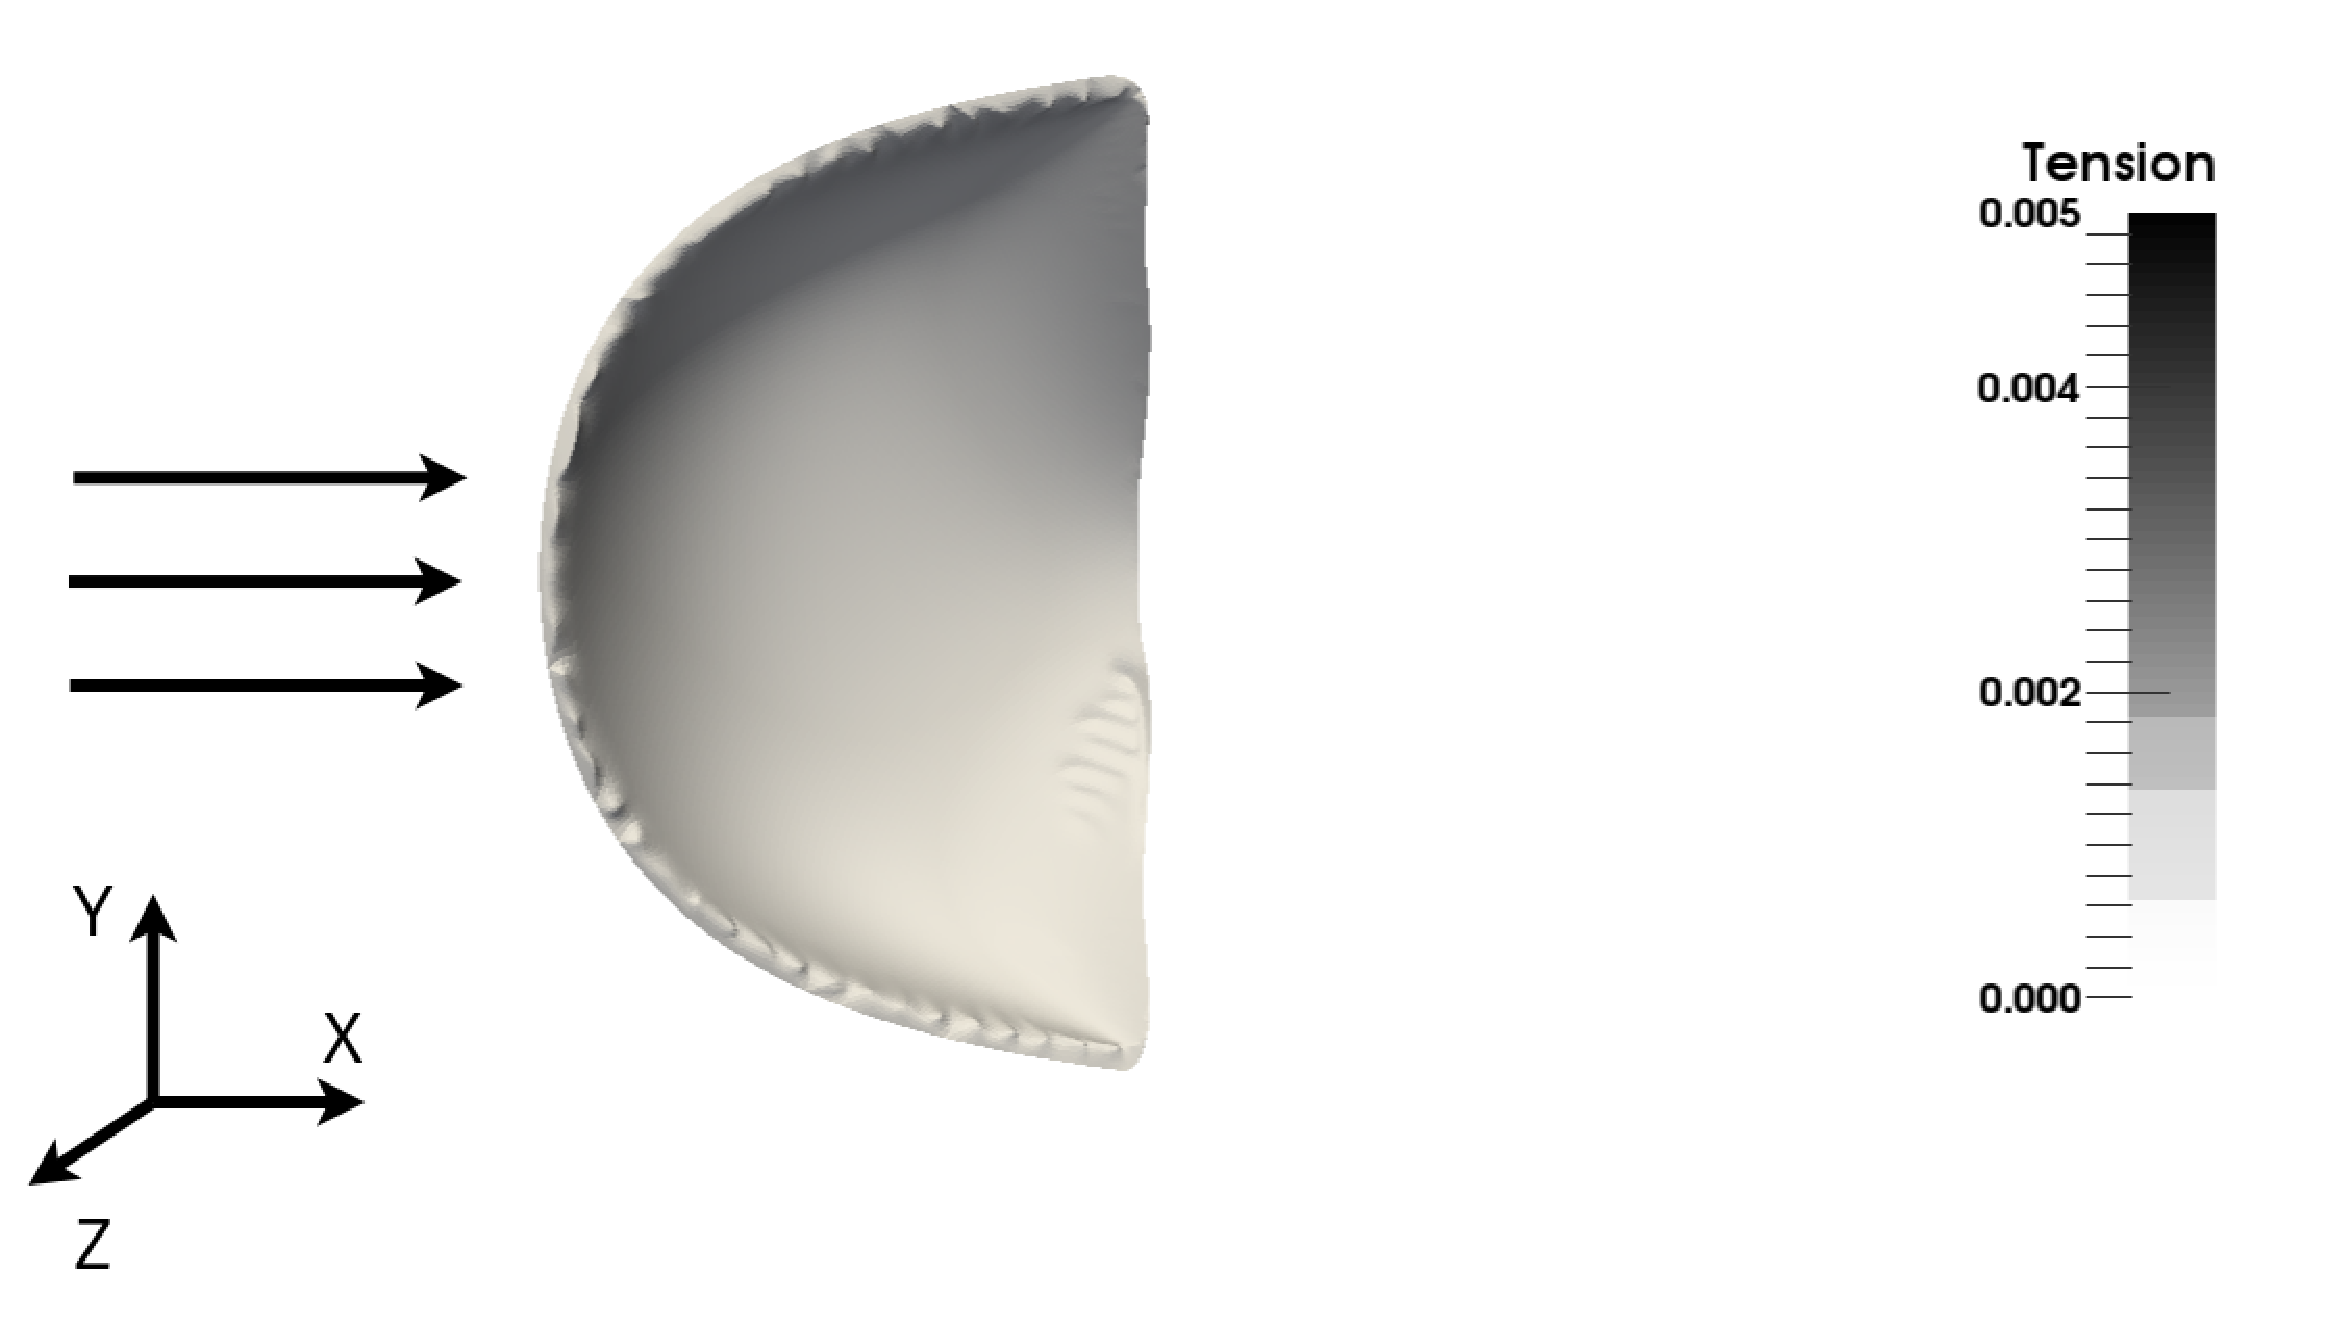
\includegraphics[width=8.5cm]{ideal_valve_stress_1_better_axes.eps}

a

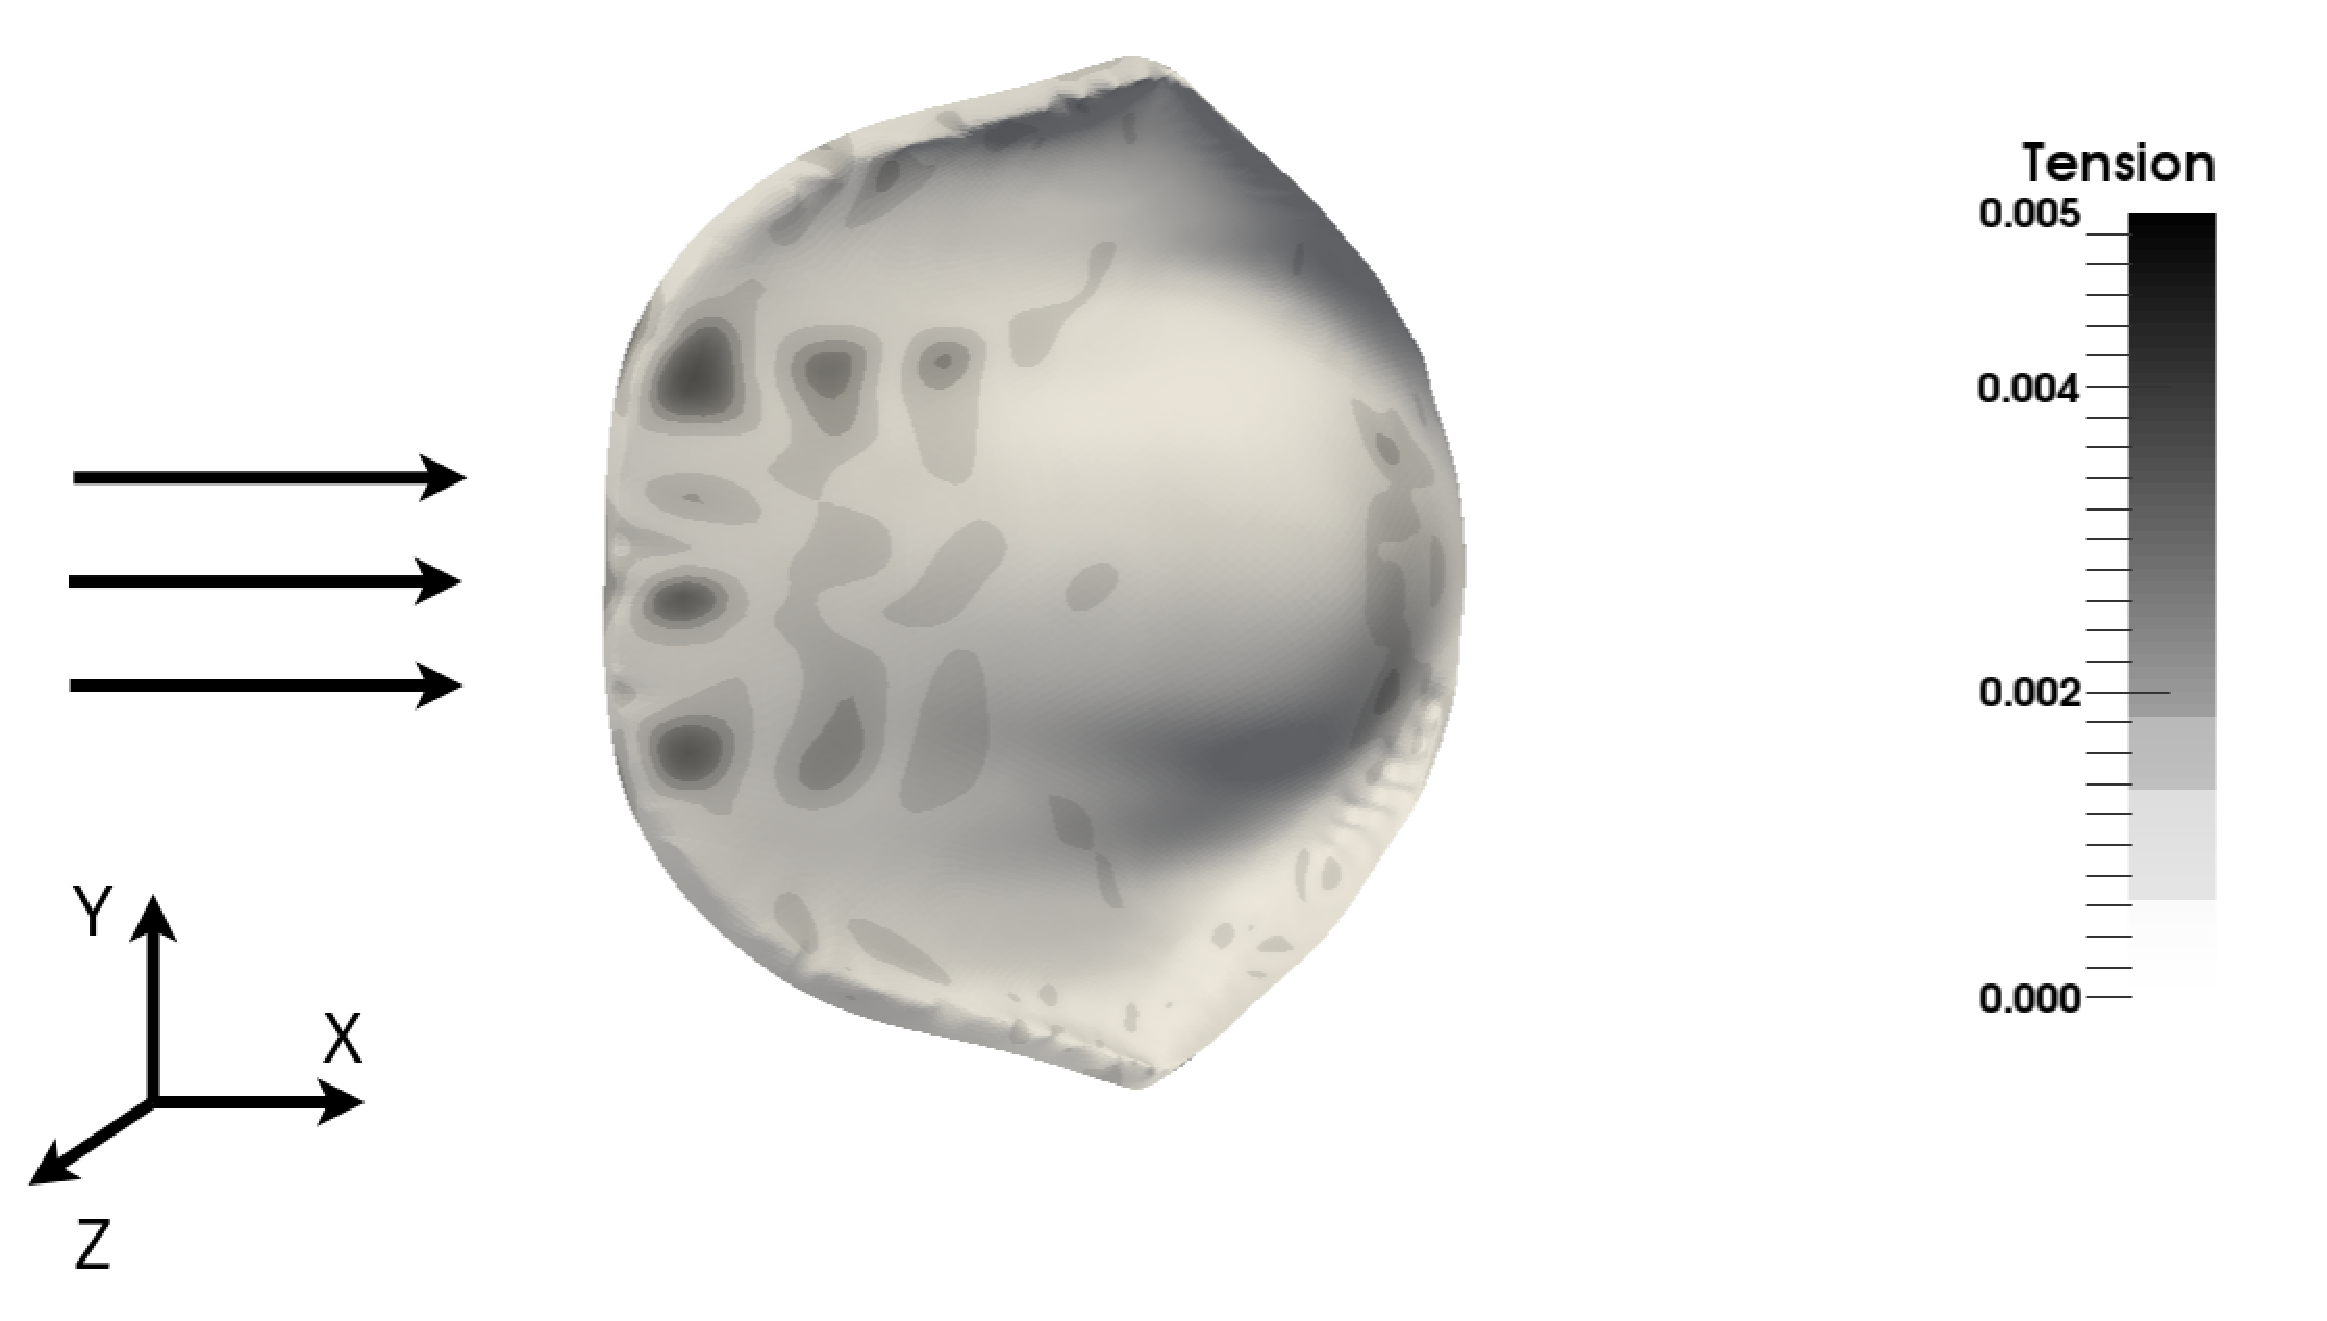
\includegraphics[width=8.5cm]{ideal_valve_stress_2_better_axes.eps}

b

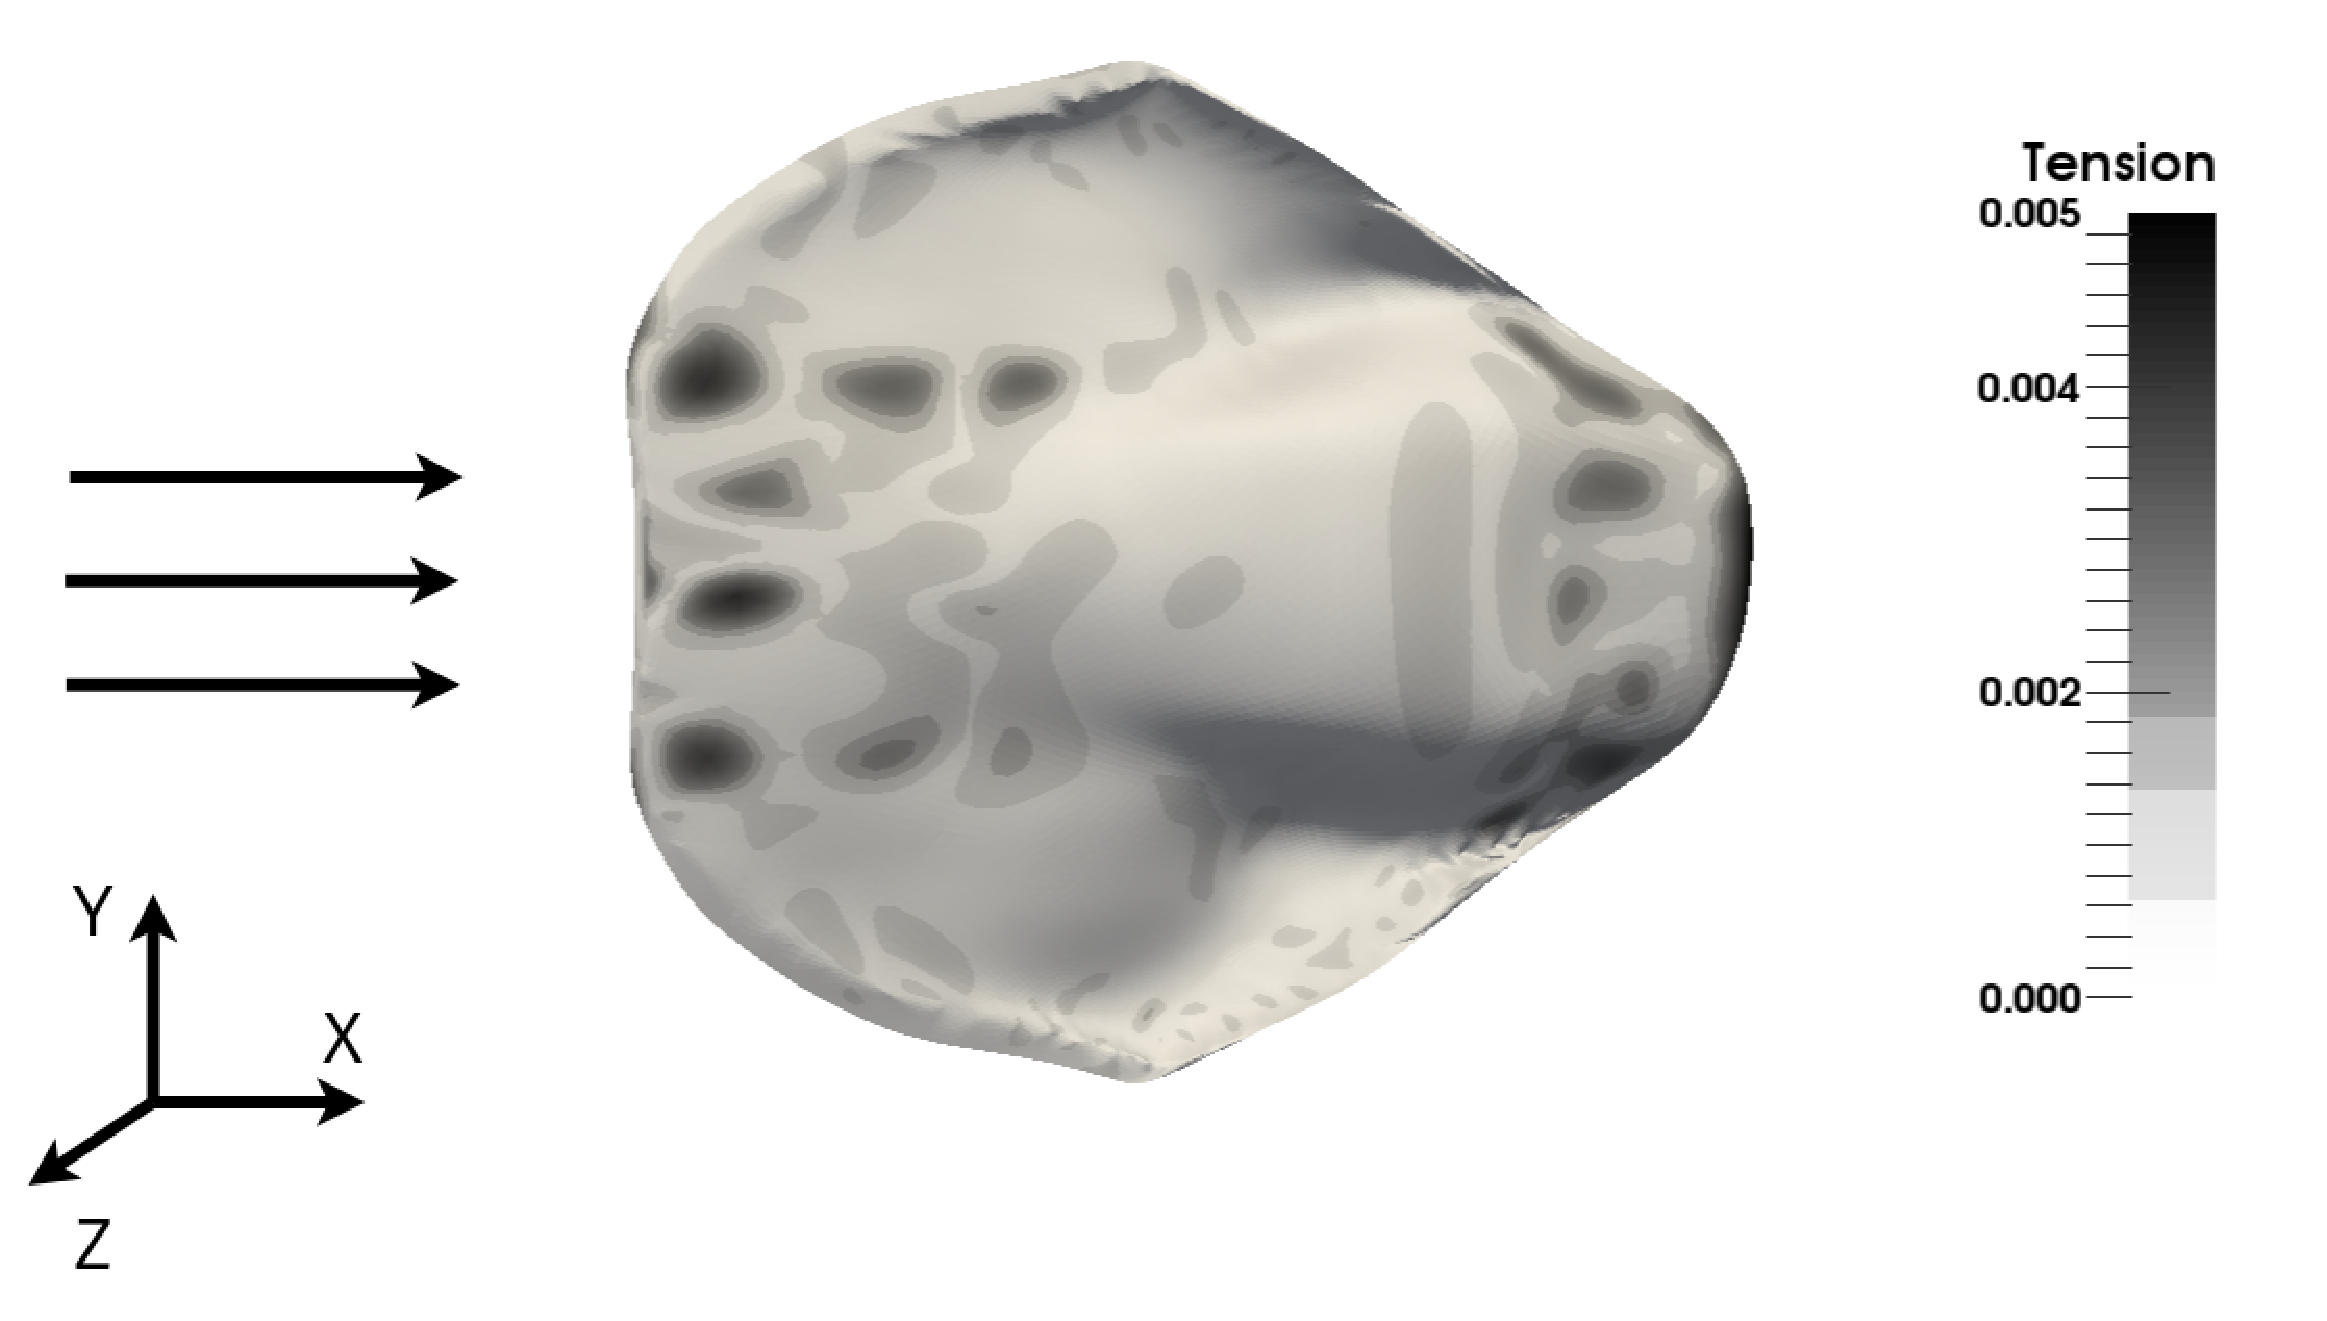
\includegraphics[width=8.5cm]{ideal_valve_stress_3_better_axes.eps}

c

\caption{Распределение напряжение по поверхности створки в моменты времени $t=0,
    t=0.4, t=0.8$. Точками обозначены стенки сосуда}
\label{fig:ideal_valve_stress}
\end{figure}

Как видно из рис. \ref{fig:ideal_valve_stress}, больше поверхностного
напряжения возникает в двух областях - на конце створки, т.к. это самая
гибкая его часть, которая подвержена наибольшим деформациям скручивания,
и в области крепления створки к фиброзному кольцу, т.к. там возникает
наибольшая деформация растяжения в силу фиксированного расположения.

На рис. \ref{fig:uniline_dynamics} представлена динамика движения для
клапана ''Юнилайн'', который двигается под воздействием движения
жидкости.

\begin{figure}[!htbp]
\centering
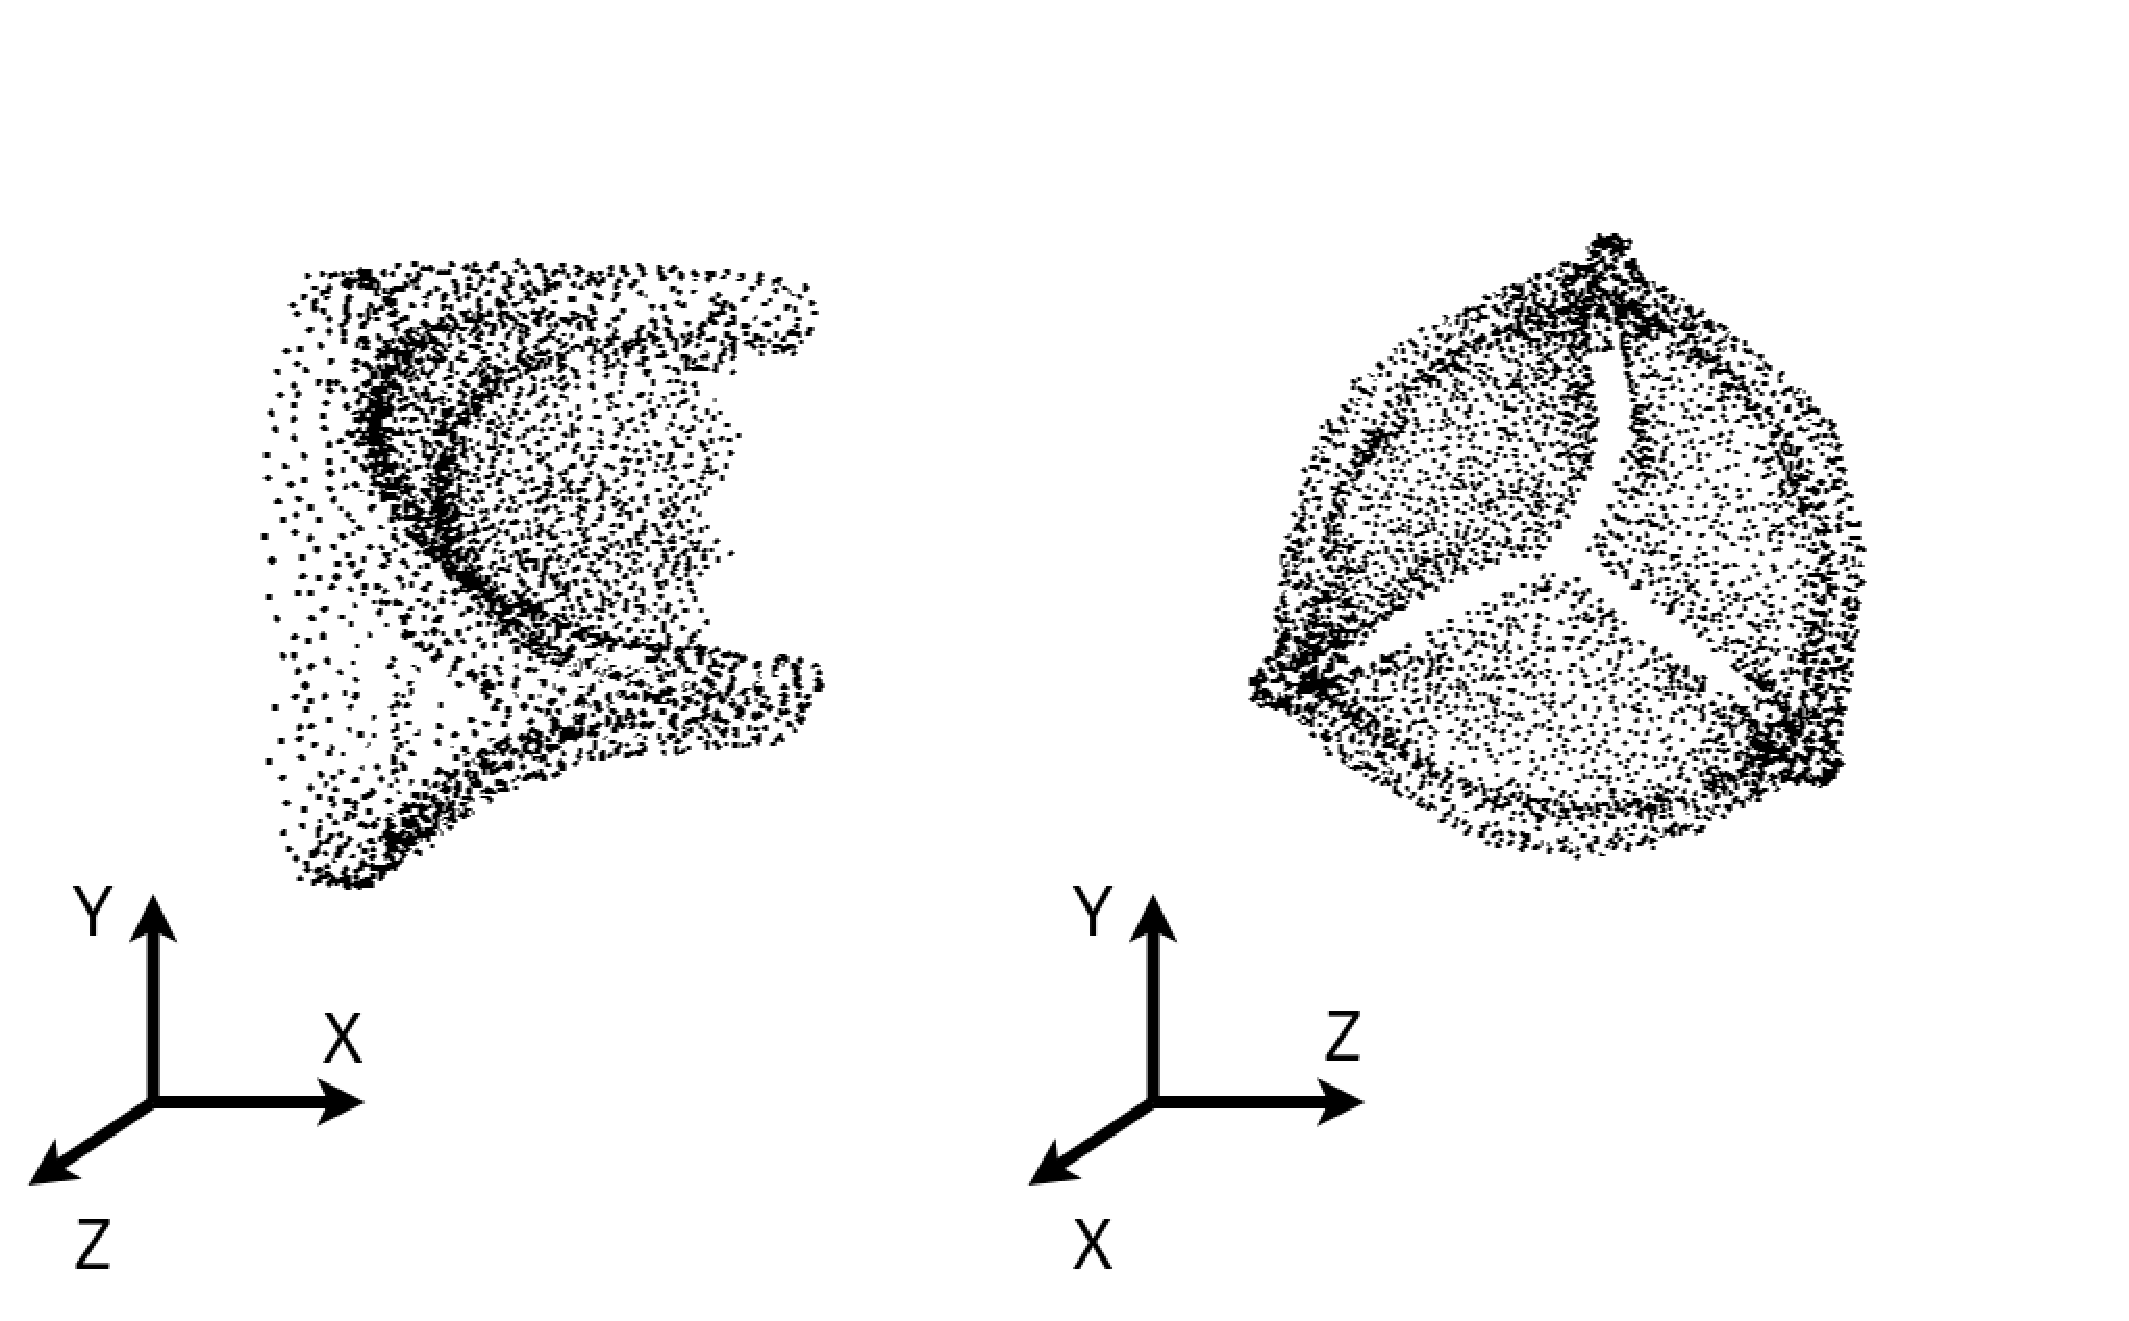
\includegraphics[width=8.5cm]{uniline_dynamics_11_axes.eps}

a

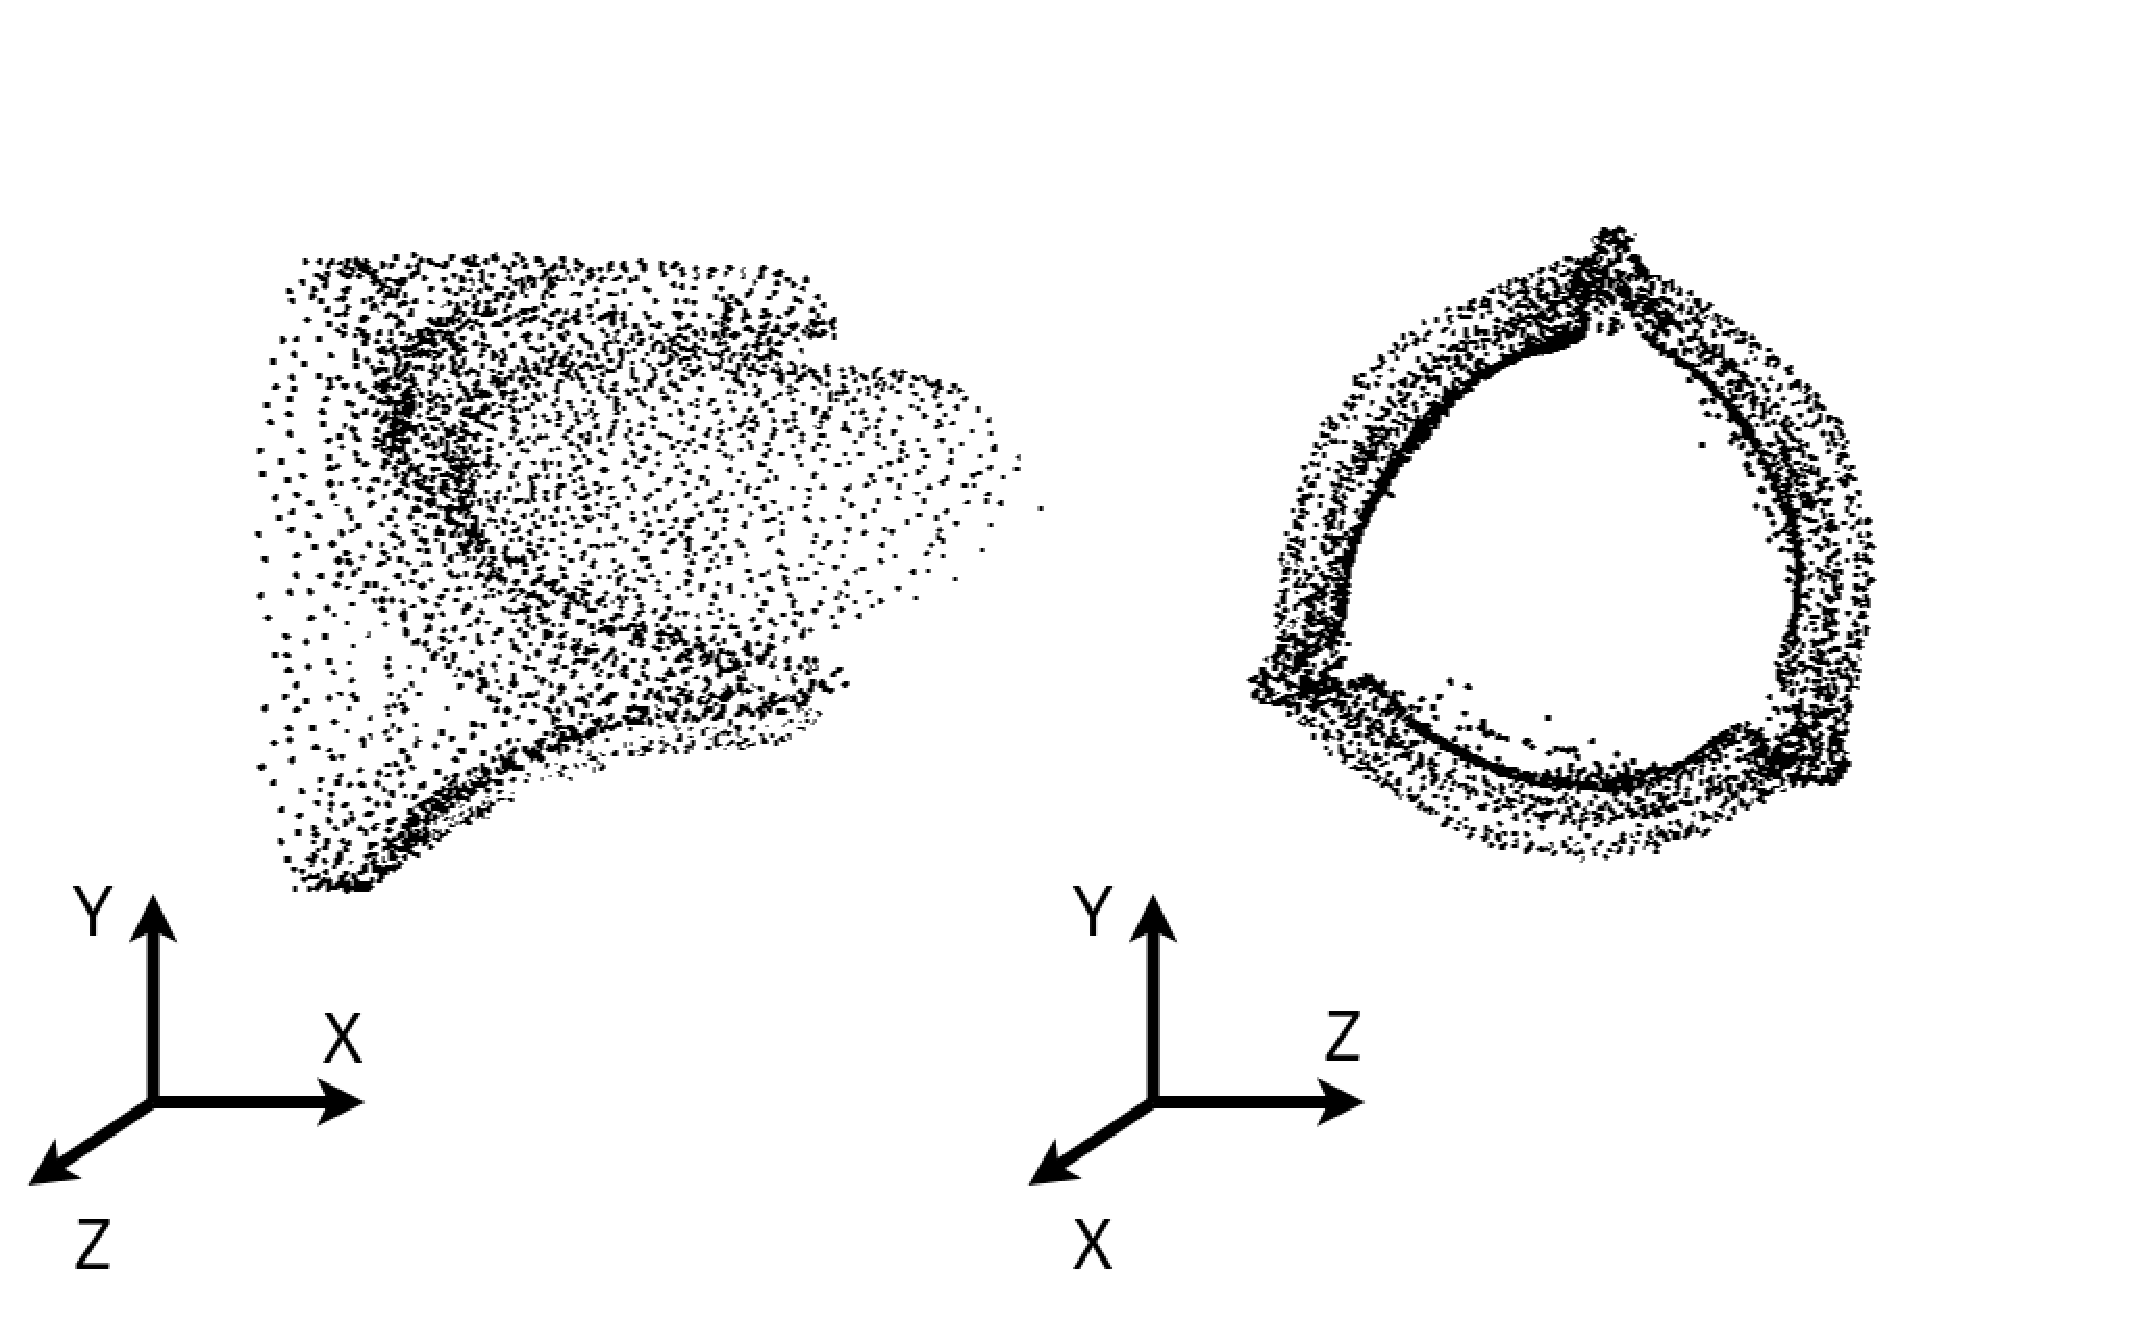
\includegraphics[width=8.5cm]{uniline_dynamics_22_axes.eps}

b

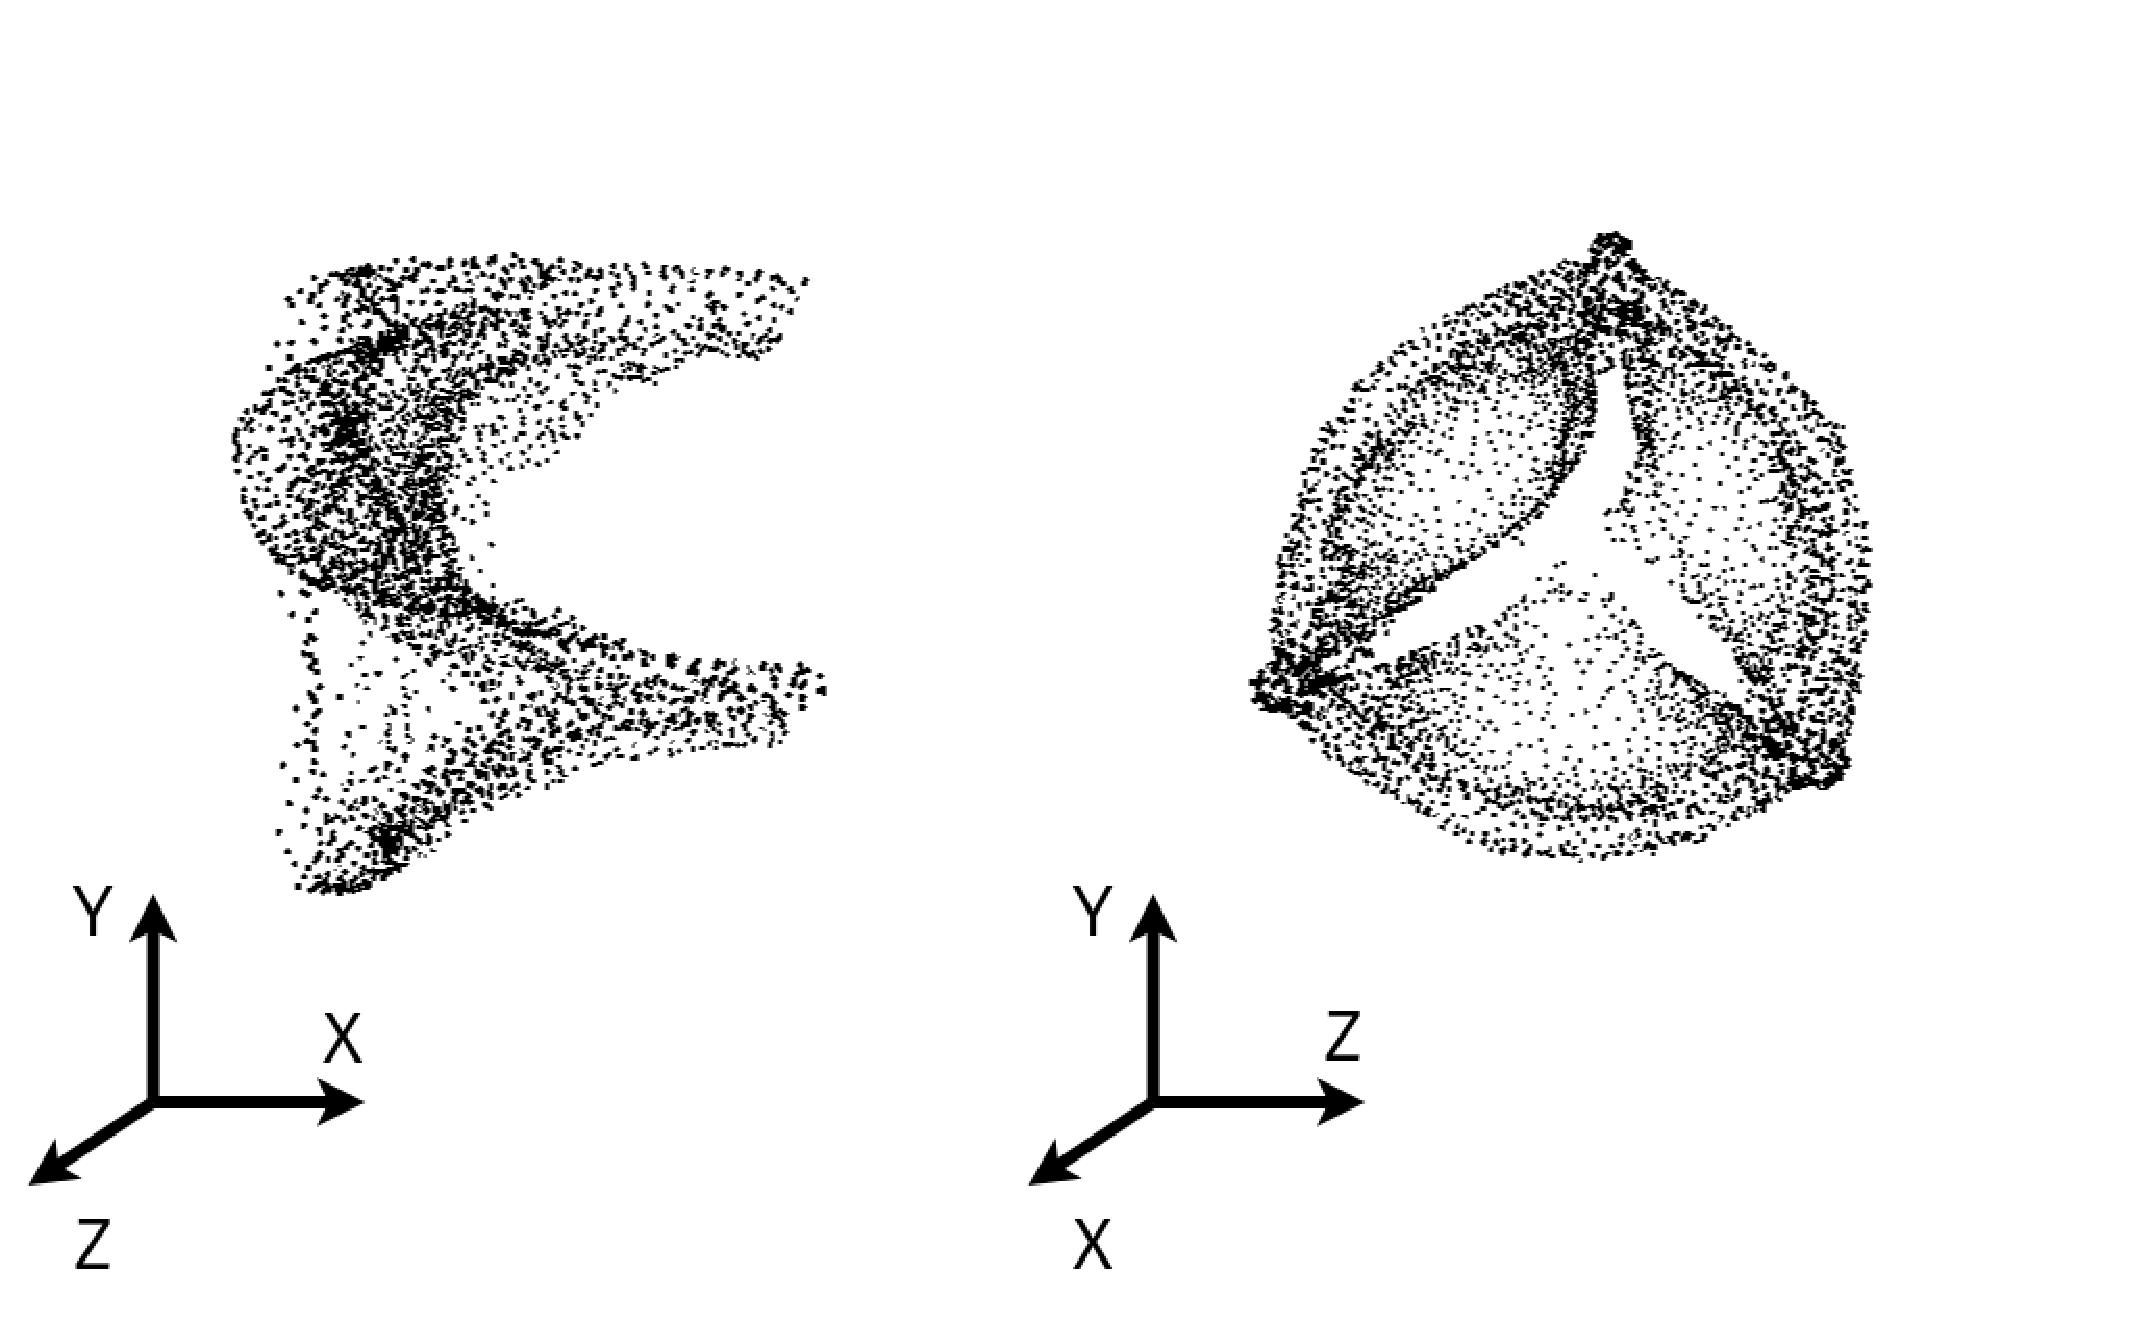
\includegraphics[width=8.5cm]{uniline_dynamics_33_axes.eps}

c

\caption{Работа клапана в моменты времени $t=0, t=0.5, t=1.8$. Точками обозначена
    поверхность фиброзного кольца и створки клапана}
\label{fig:uniline_dynamics}
\end{figure}

На рис. \ref{fig:uniline_stress} представлена динамика движения и
распределение поверхностного напряжения для створки клапана
``Юнилайн'', который двигается под воздействием движения жидкости с
переменной вязкостью и плотностью
\(\rho_1=1, \rho_2=2, \mu_1=1 \cdot 10^{-2}, \mu_2=2 \cdot 10^{-2}\).

\begin{figure}[!htbp]
\centering
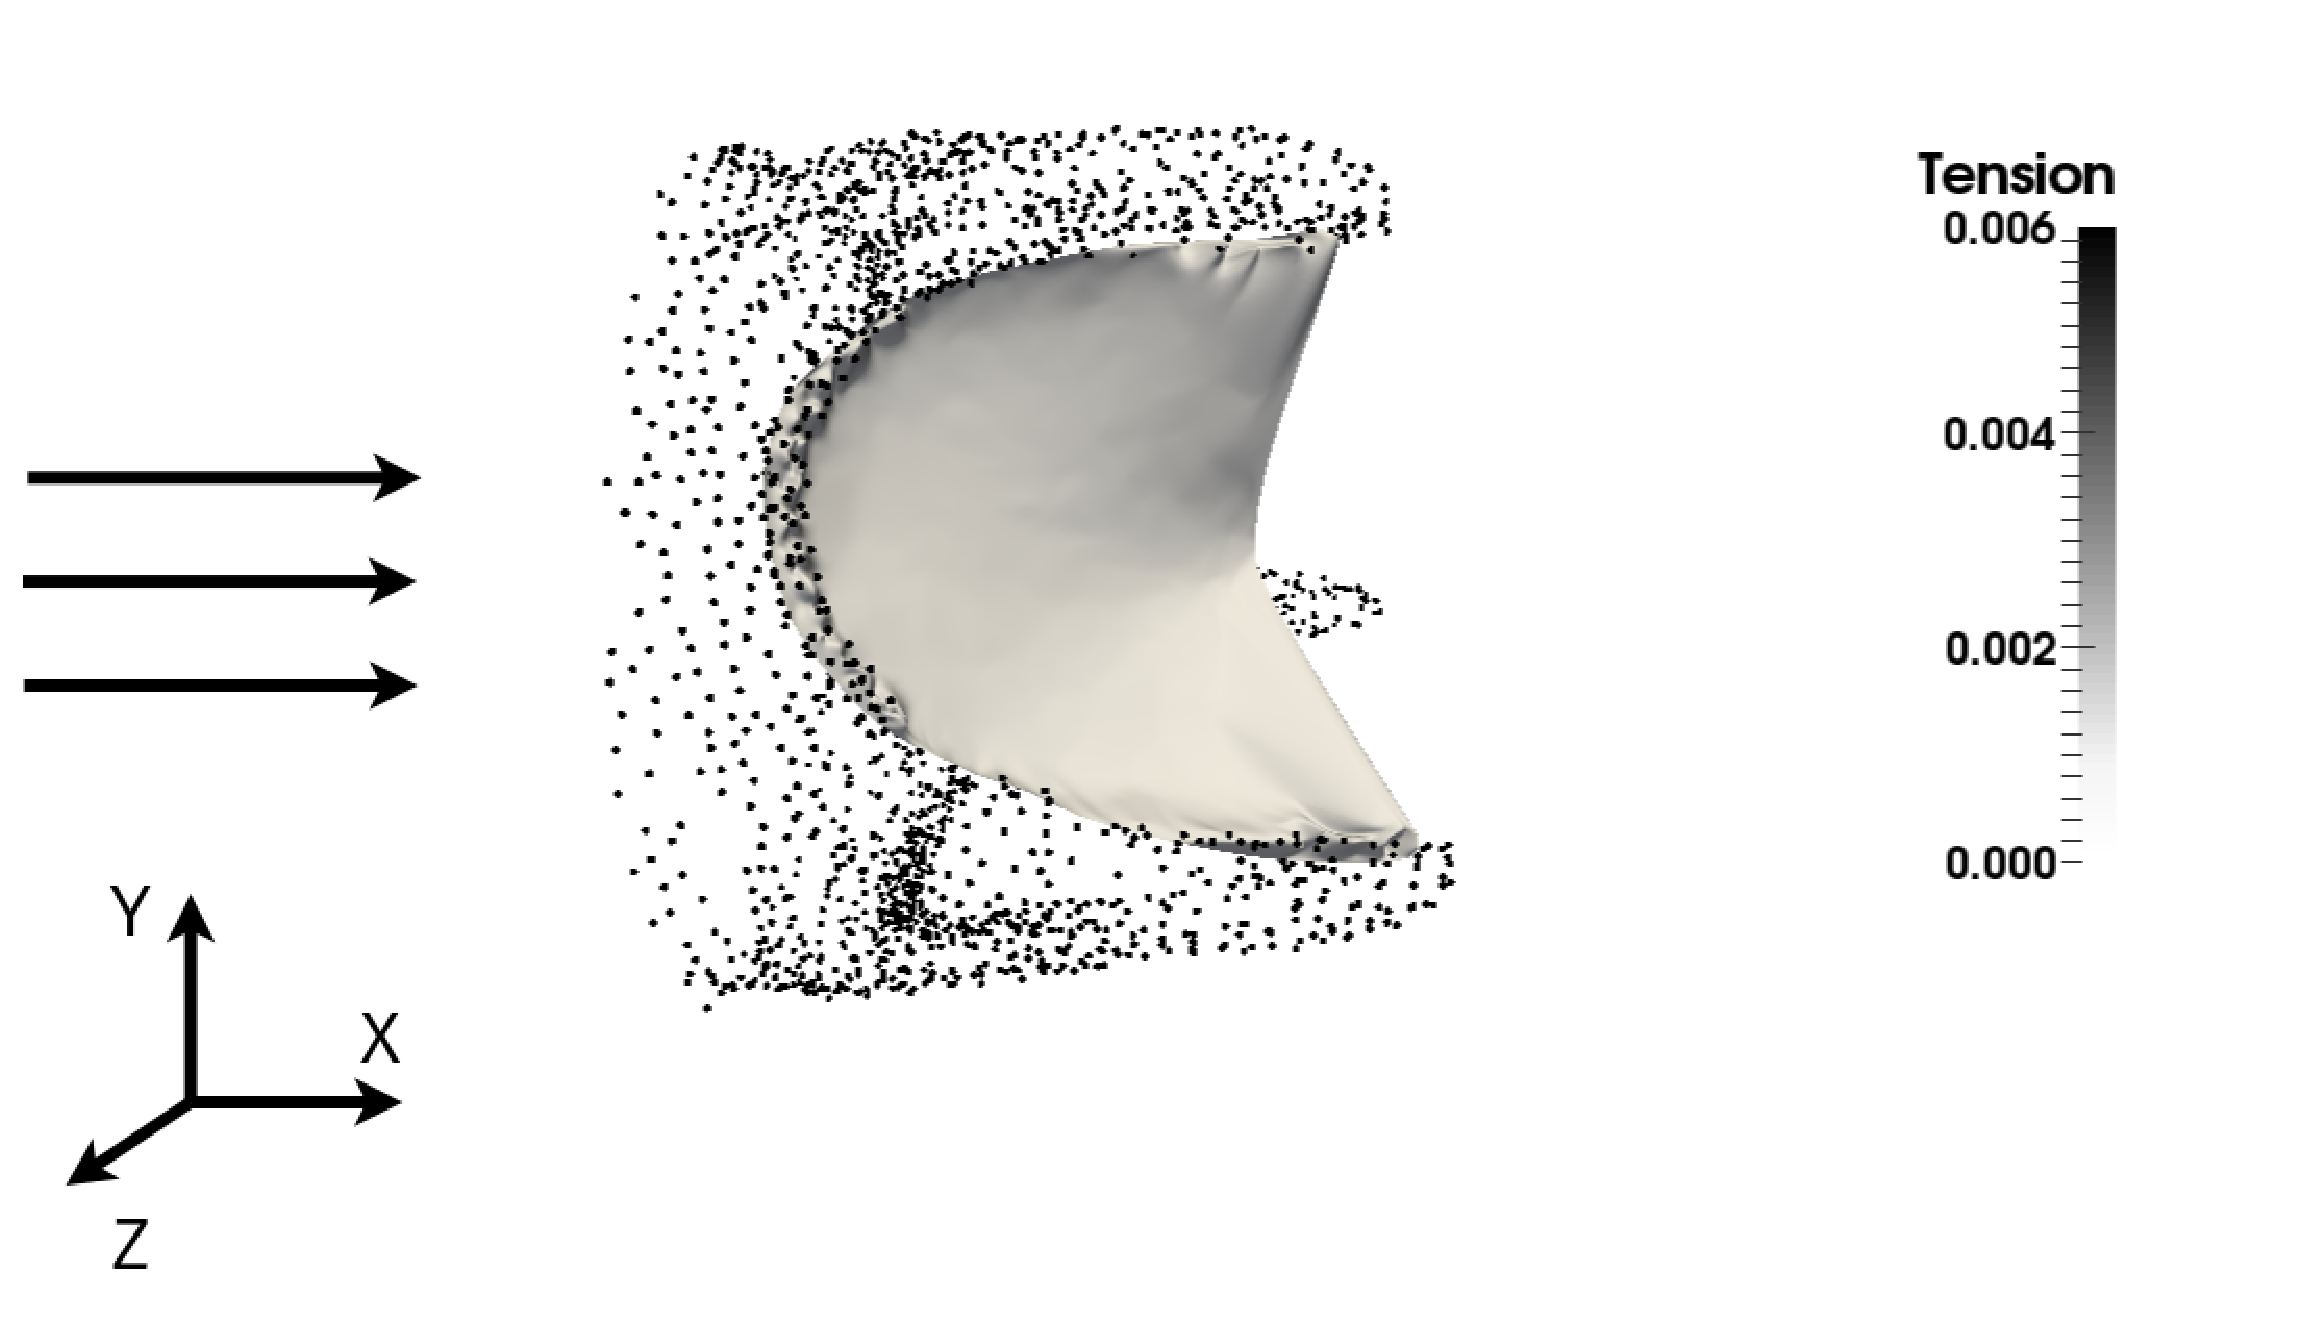
\includegraphics[width=8.5cm]{uniline_stress_1_better_axes.eps}

a

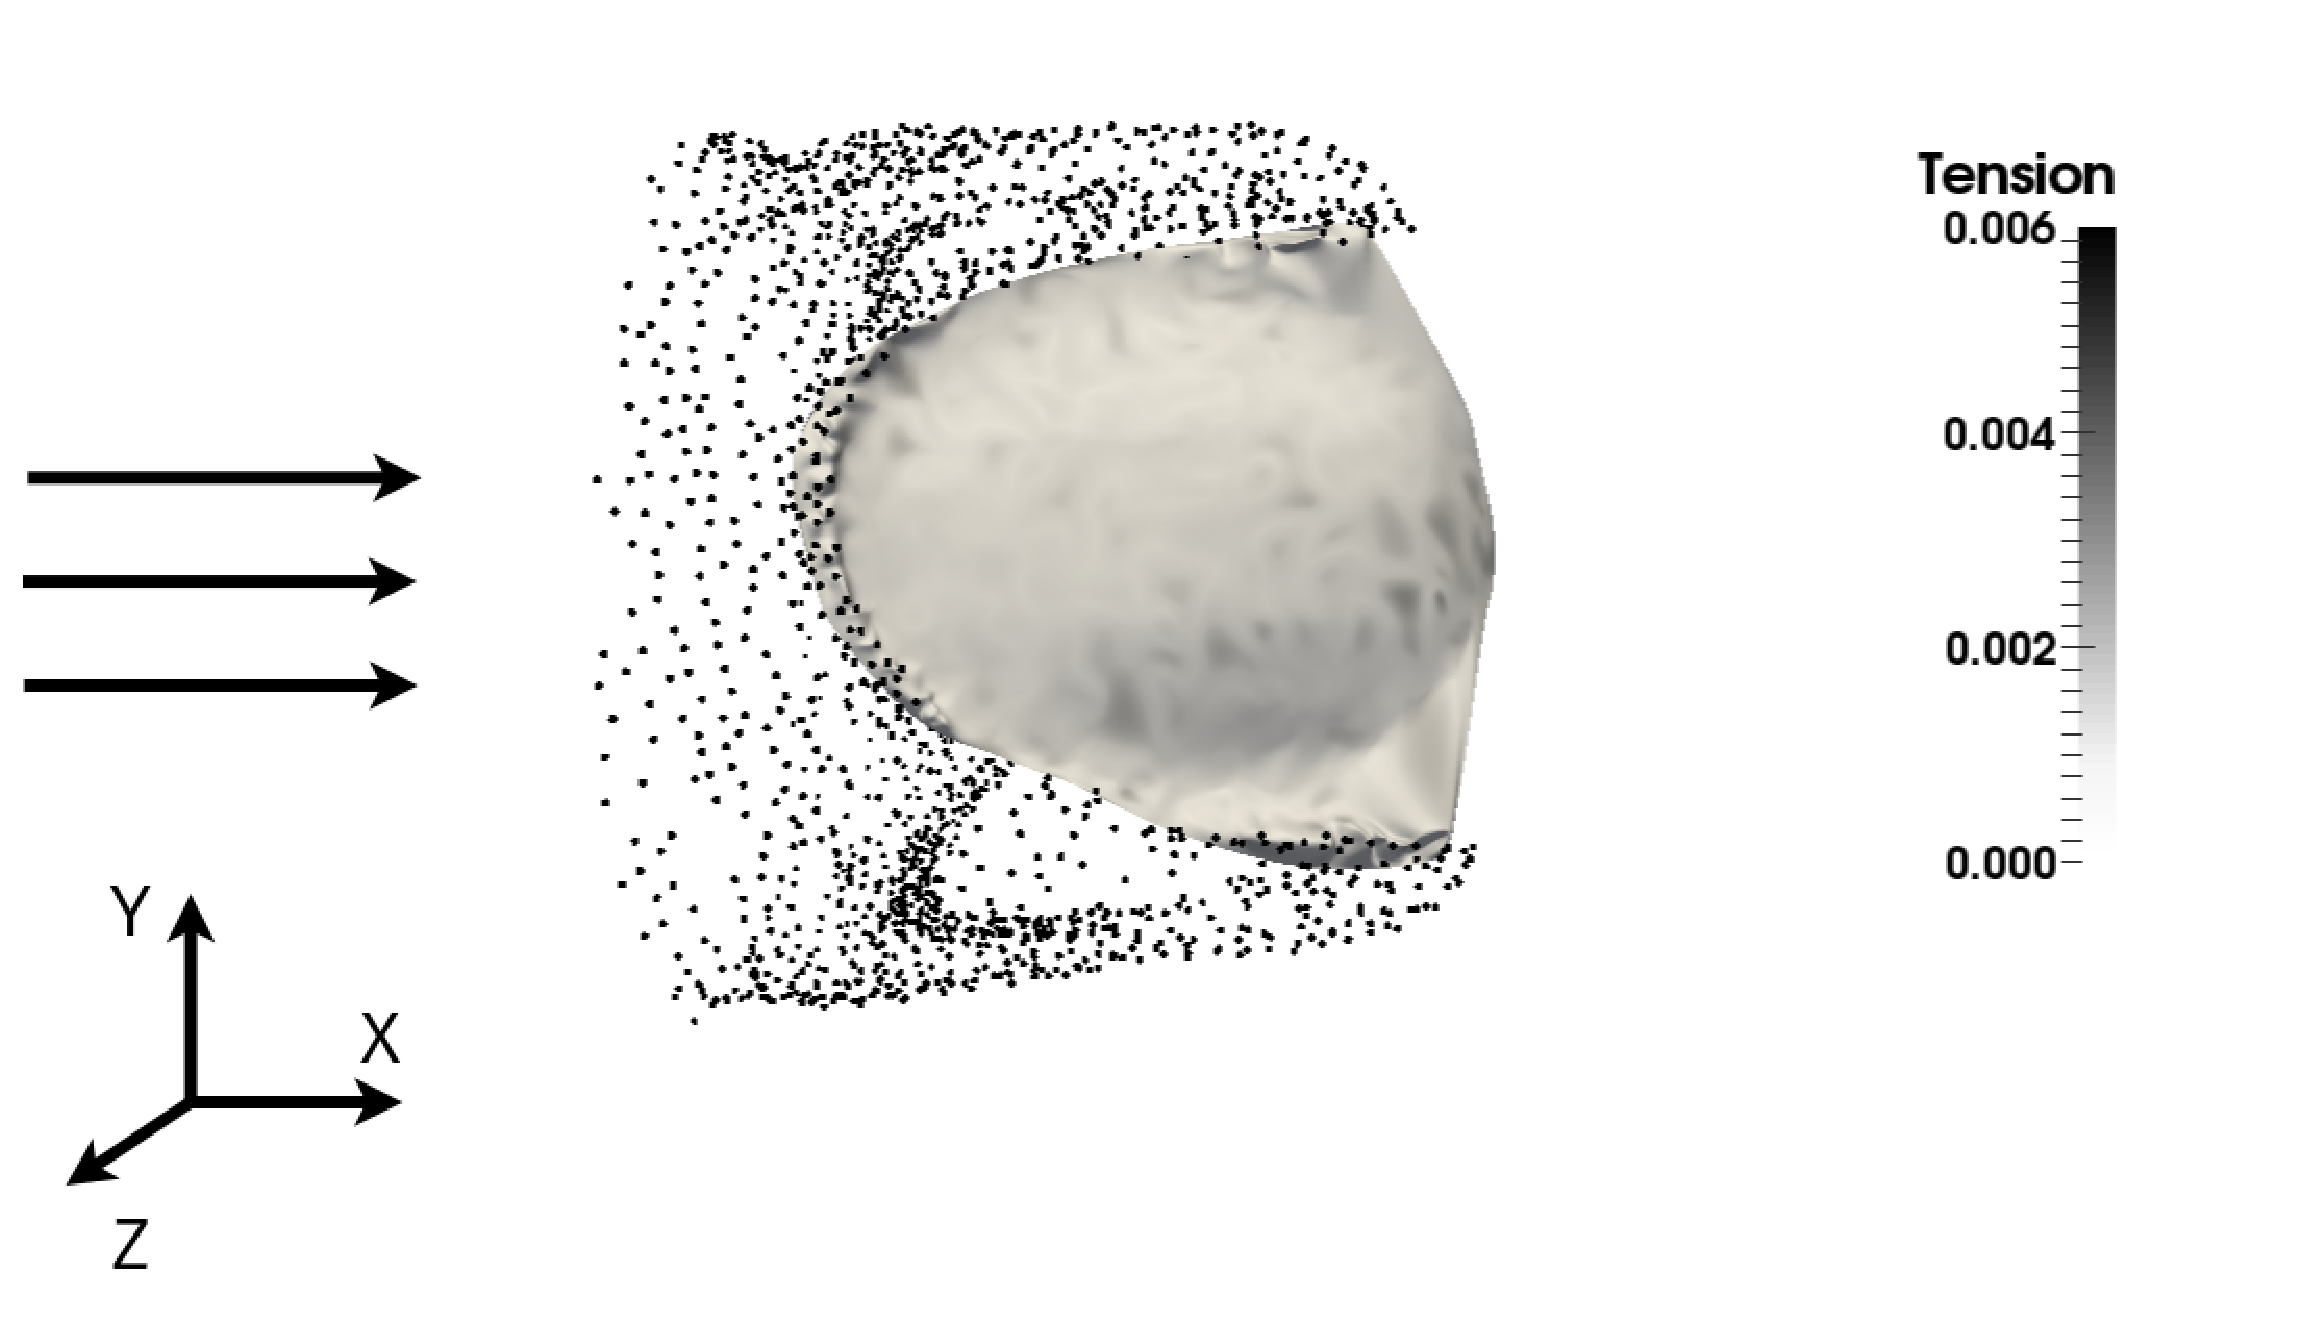
\includegraphics[width=8.5cm]{uniline_stress_2_better_axes.eps}

b

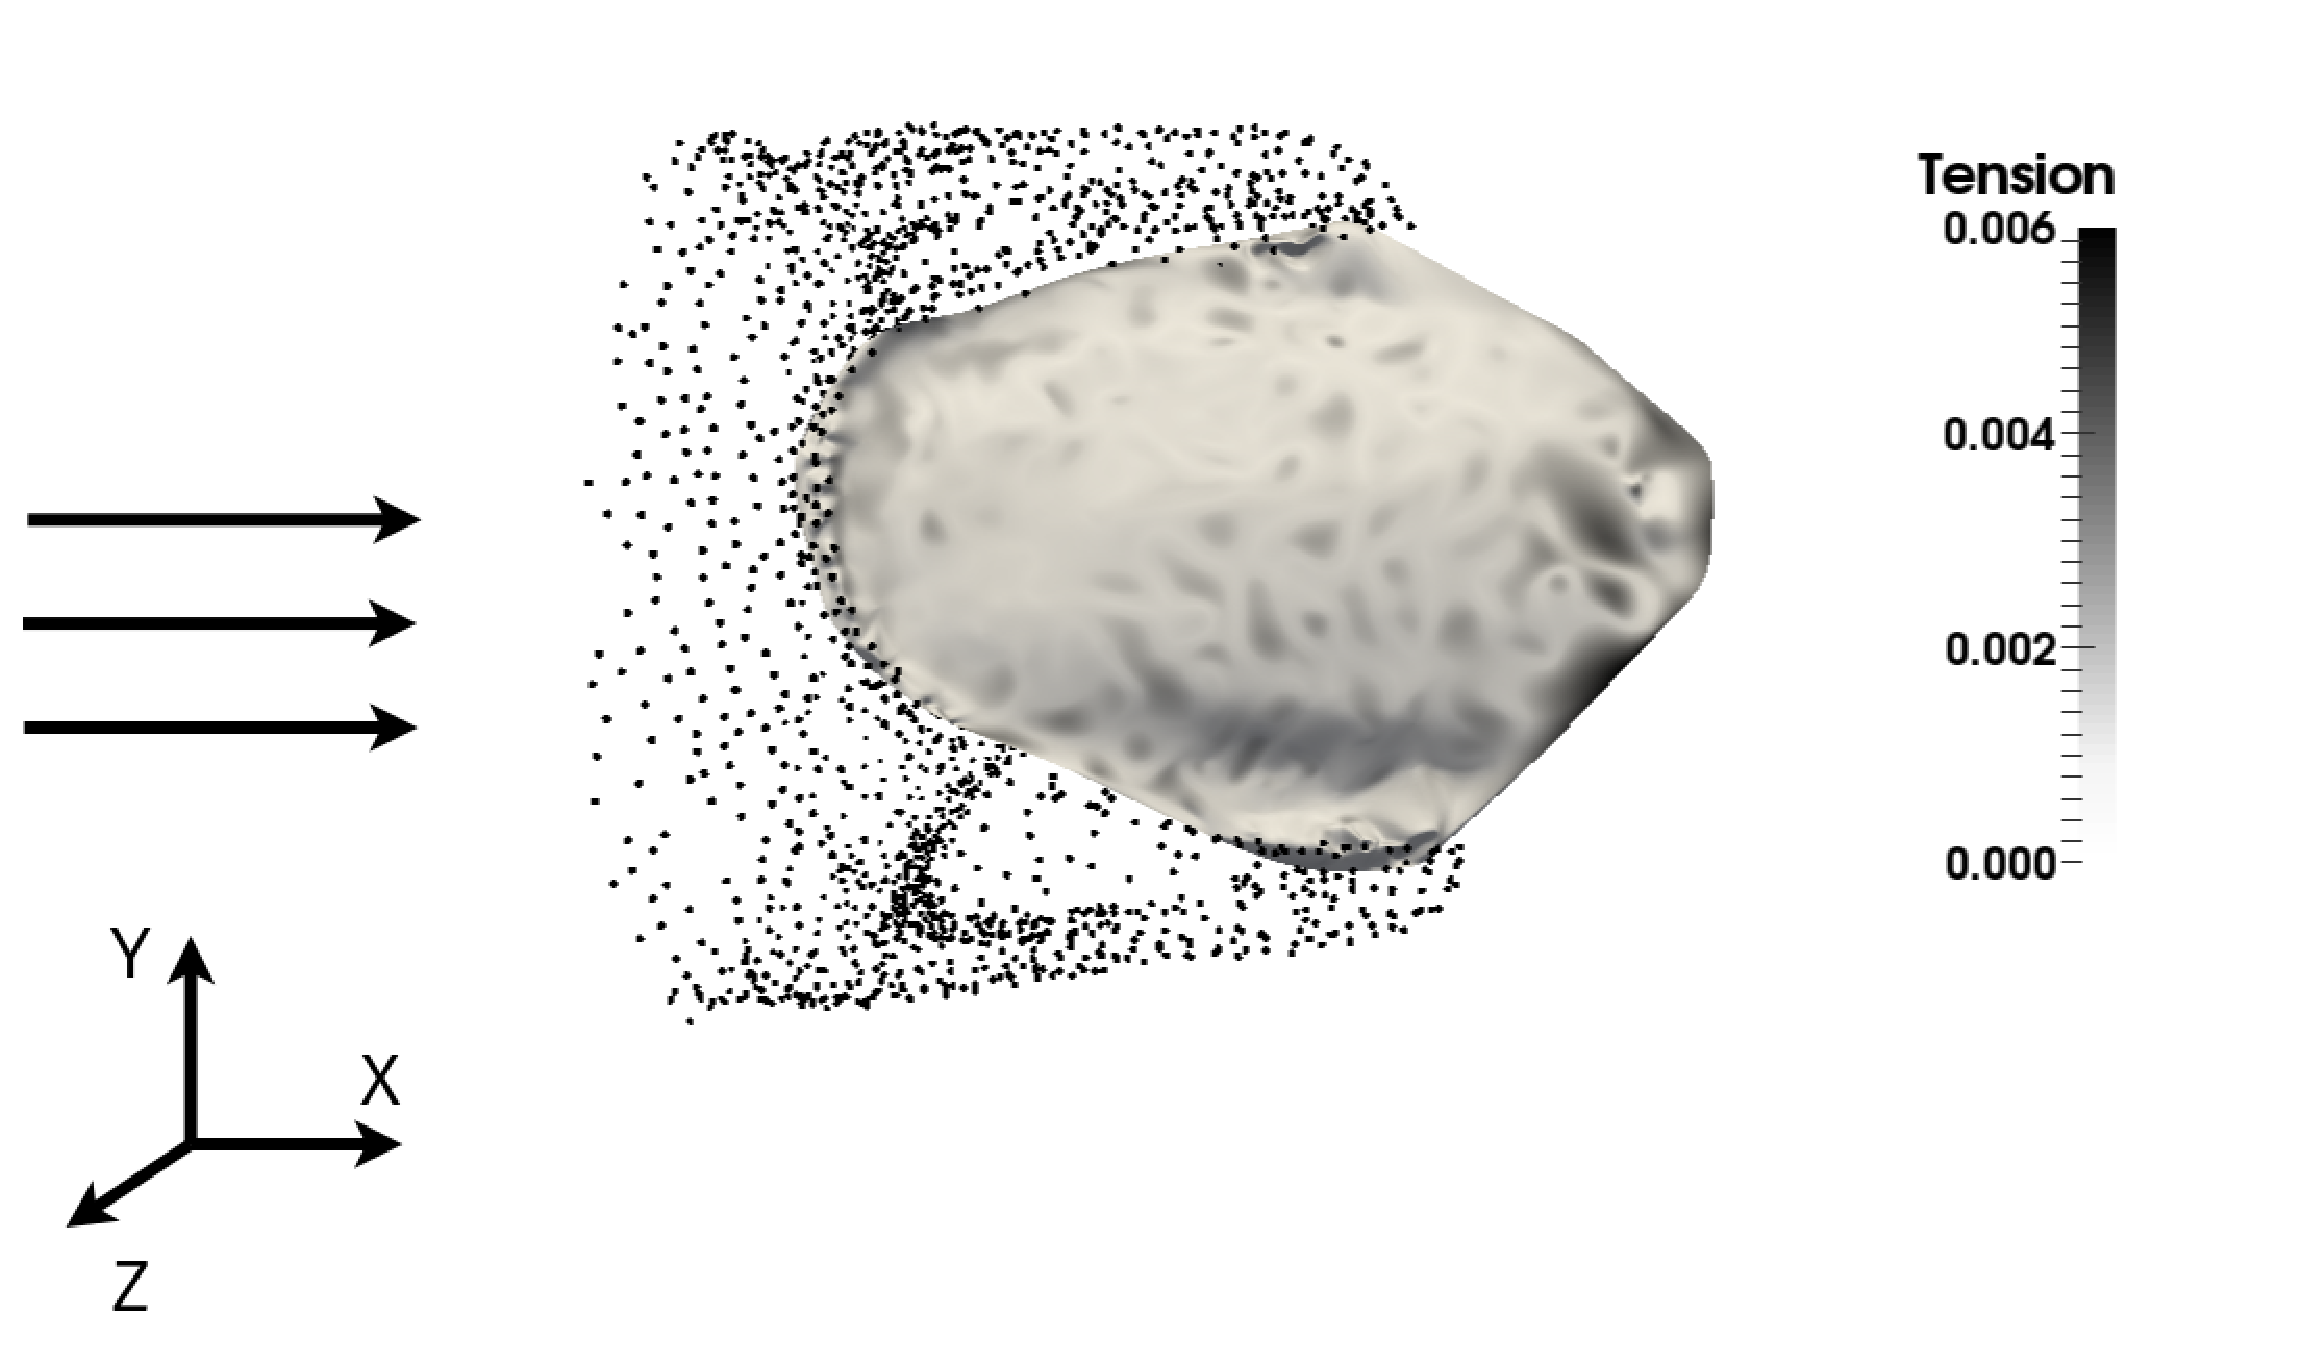
\includegraphics[width=8.5cm]{uniline_stress_3_better_axes.eps}

c

\caption{Распределение напряжение по поверхности одной створки в моменты времени $t=0,
    t=0.4, t=0.8$. Точками обозначена поверхность фиброзного кольца}
\label{fig:uniline_stress}
\end{figure}

Как видно из сравнения рис. \ref{fig:ideal_valve_stress} и рис. \ref{fig:uniline_stress},
в отличии от клапана идеальной формы, в области крепления створки ''Юнилайн'' не происходит
значительного увеличения поверхностного напряжения $F(q, r, s, t)$

Далее было решено рассмотреть влияние переменной плотности и 
вязкости на величину напряжения в трёх характерных точках клапана (см. рис. 
\ref{fig:points_scheme}): ''активная точка'',  ''пассивная точка'' и ''точка на границе''. 
''активная точка'' находится на одной из осей кольца,
рядом с областью крепления створки. ''точка на границе'' тоже
располагается в области крепления, но на удалении от осей. ''пассивная
точка'' располагается на внешней, наименее подвижной части кольца 
 
\begin{figure}[!htbp]
\centering
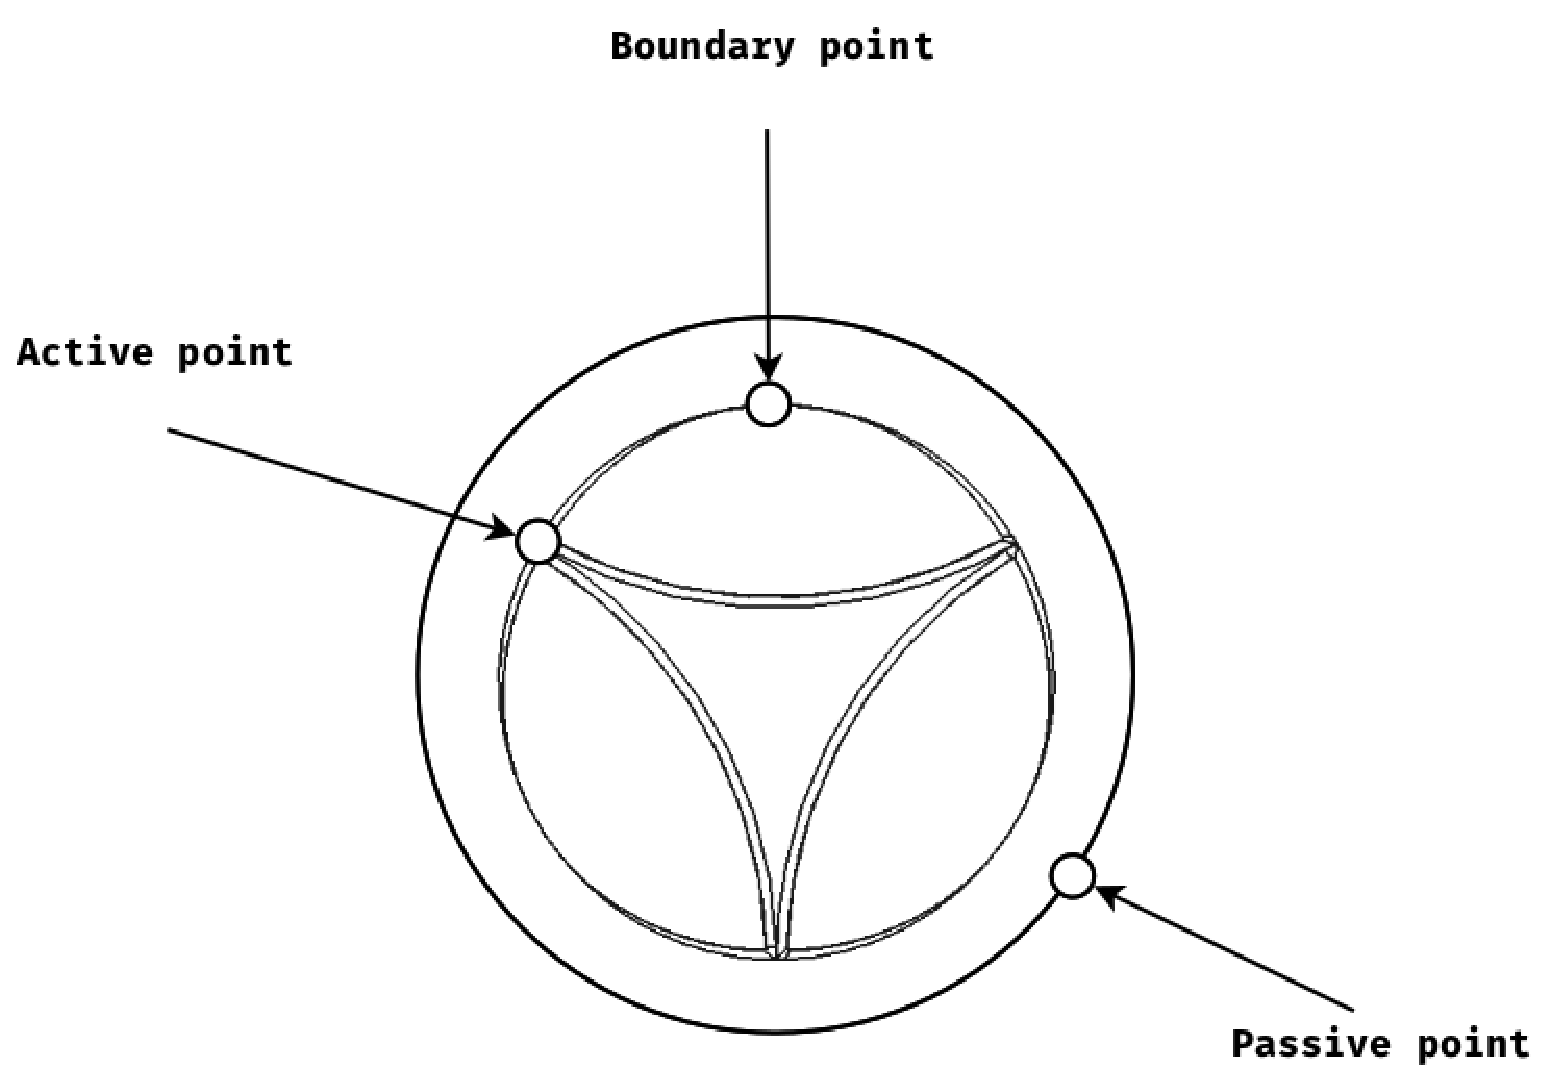
\includegraphics[width=8.5cm]{valve_points_eng.eps}
\caption{Схема расположения точек на фиброзном кольце}
\label{fig:points_scheme}
\end{figure}

На рис. \ref{fig:fibrouse_forces} показано графики зависимости
поверхностного напряжения от времени для трех точек в разных частях
фиброзного кольца для случаев с постоянной $\rho_1=\rho_2=1, \mu_1=\mu_2=1 \cdot 10^{-2}$
и переменной $\rho_1=1, \rho_2=2, \mu_1=1 \cdot 10^{-2}, \mu_2=2 \cdot 10^{-2}$ вязкостью.
(см.
рис. \ref{fig:points_scheme}).

\begin{figure}[!htbp]
\centering
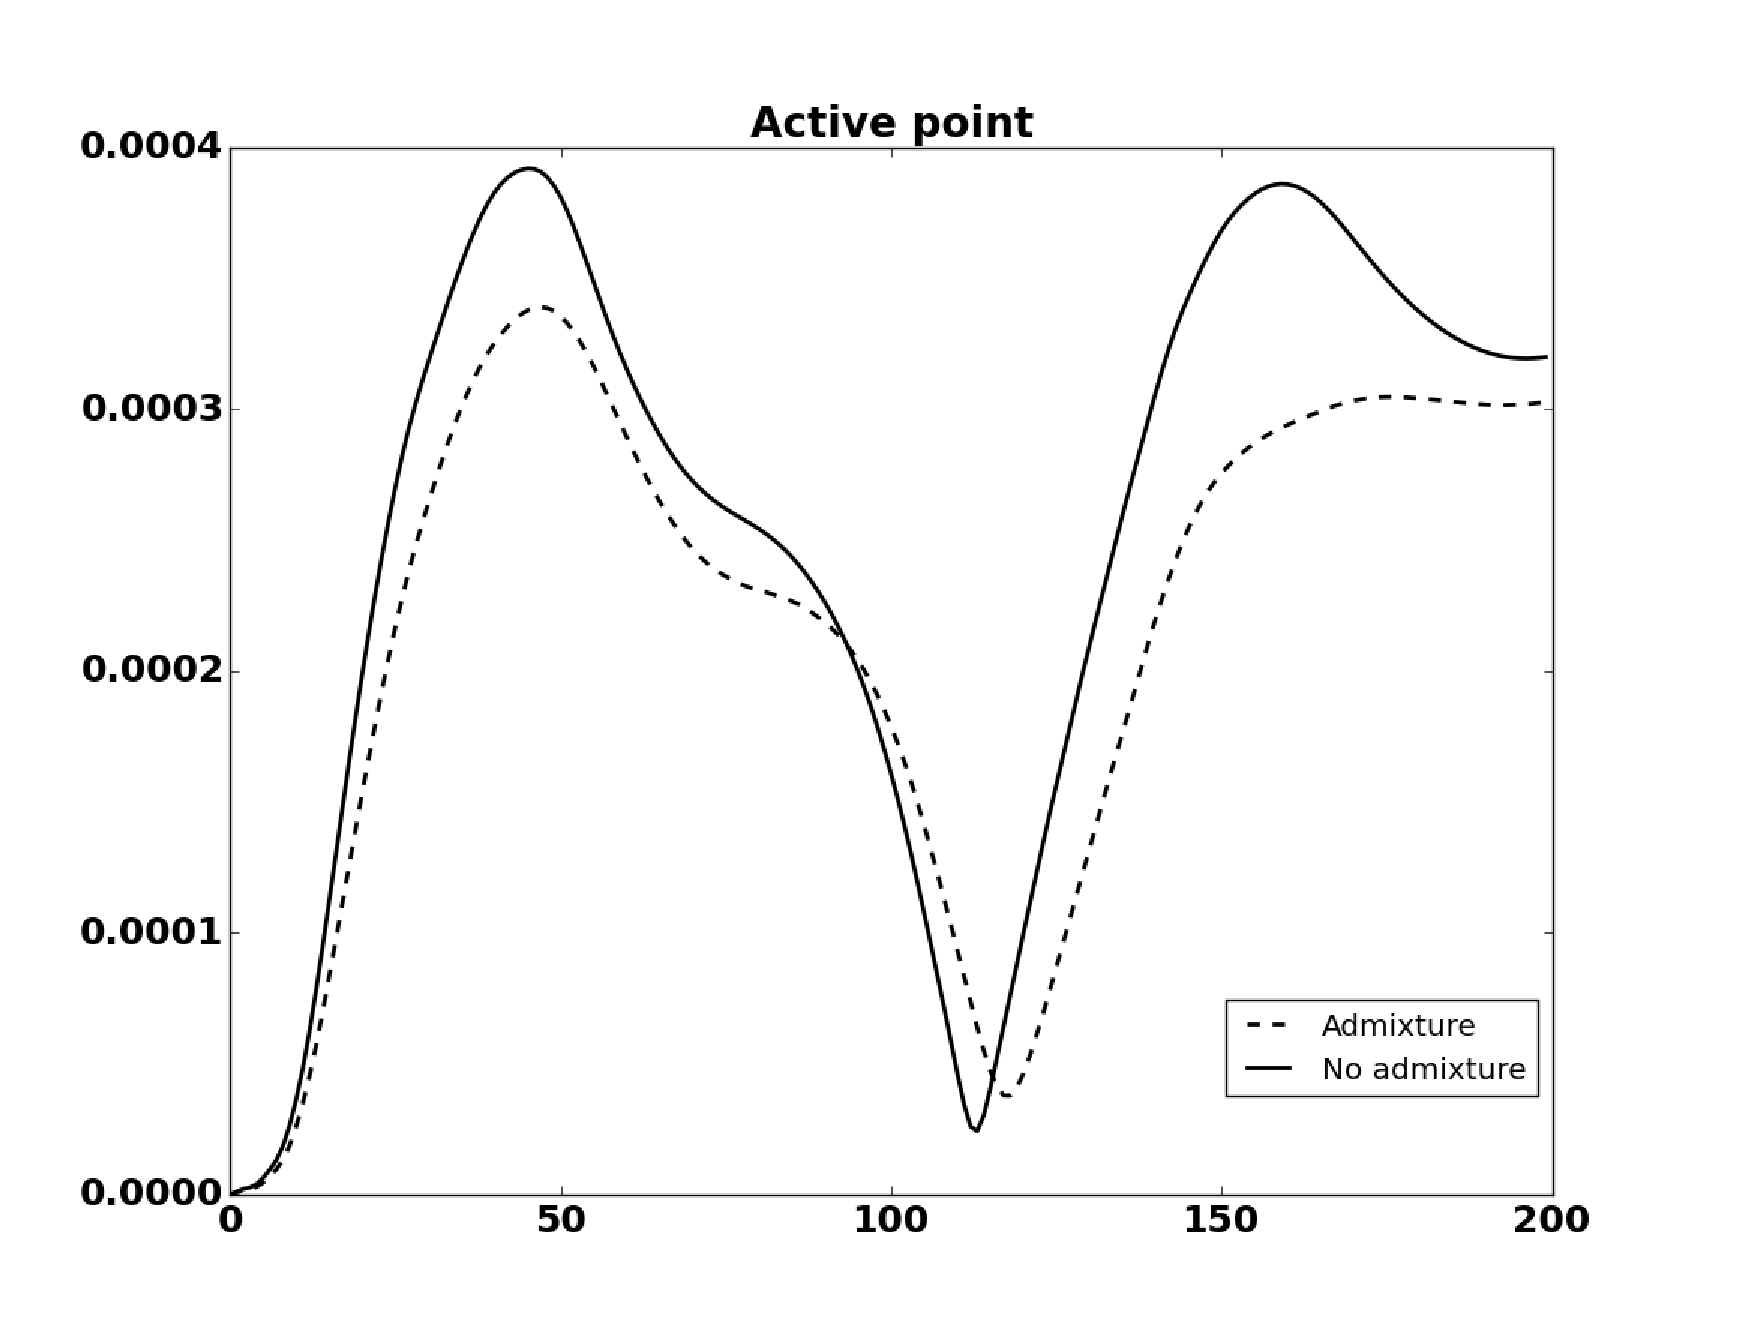
\includegraphics[width=8.5cm]{forces_active_point_eng_bold.eps}

a

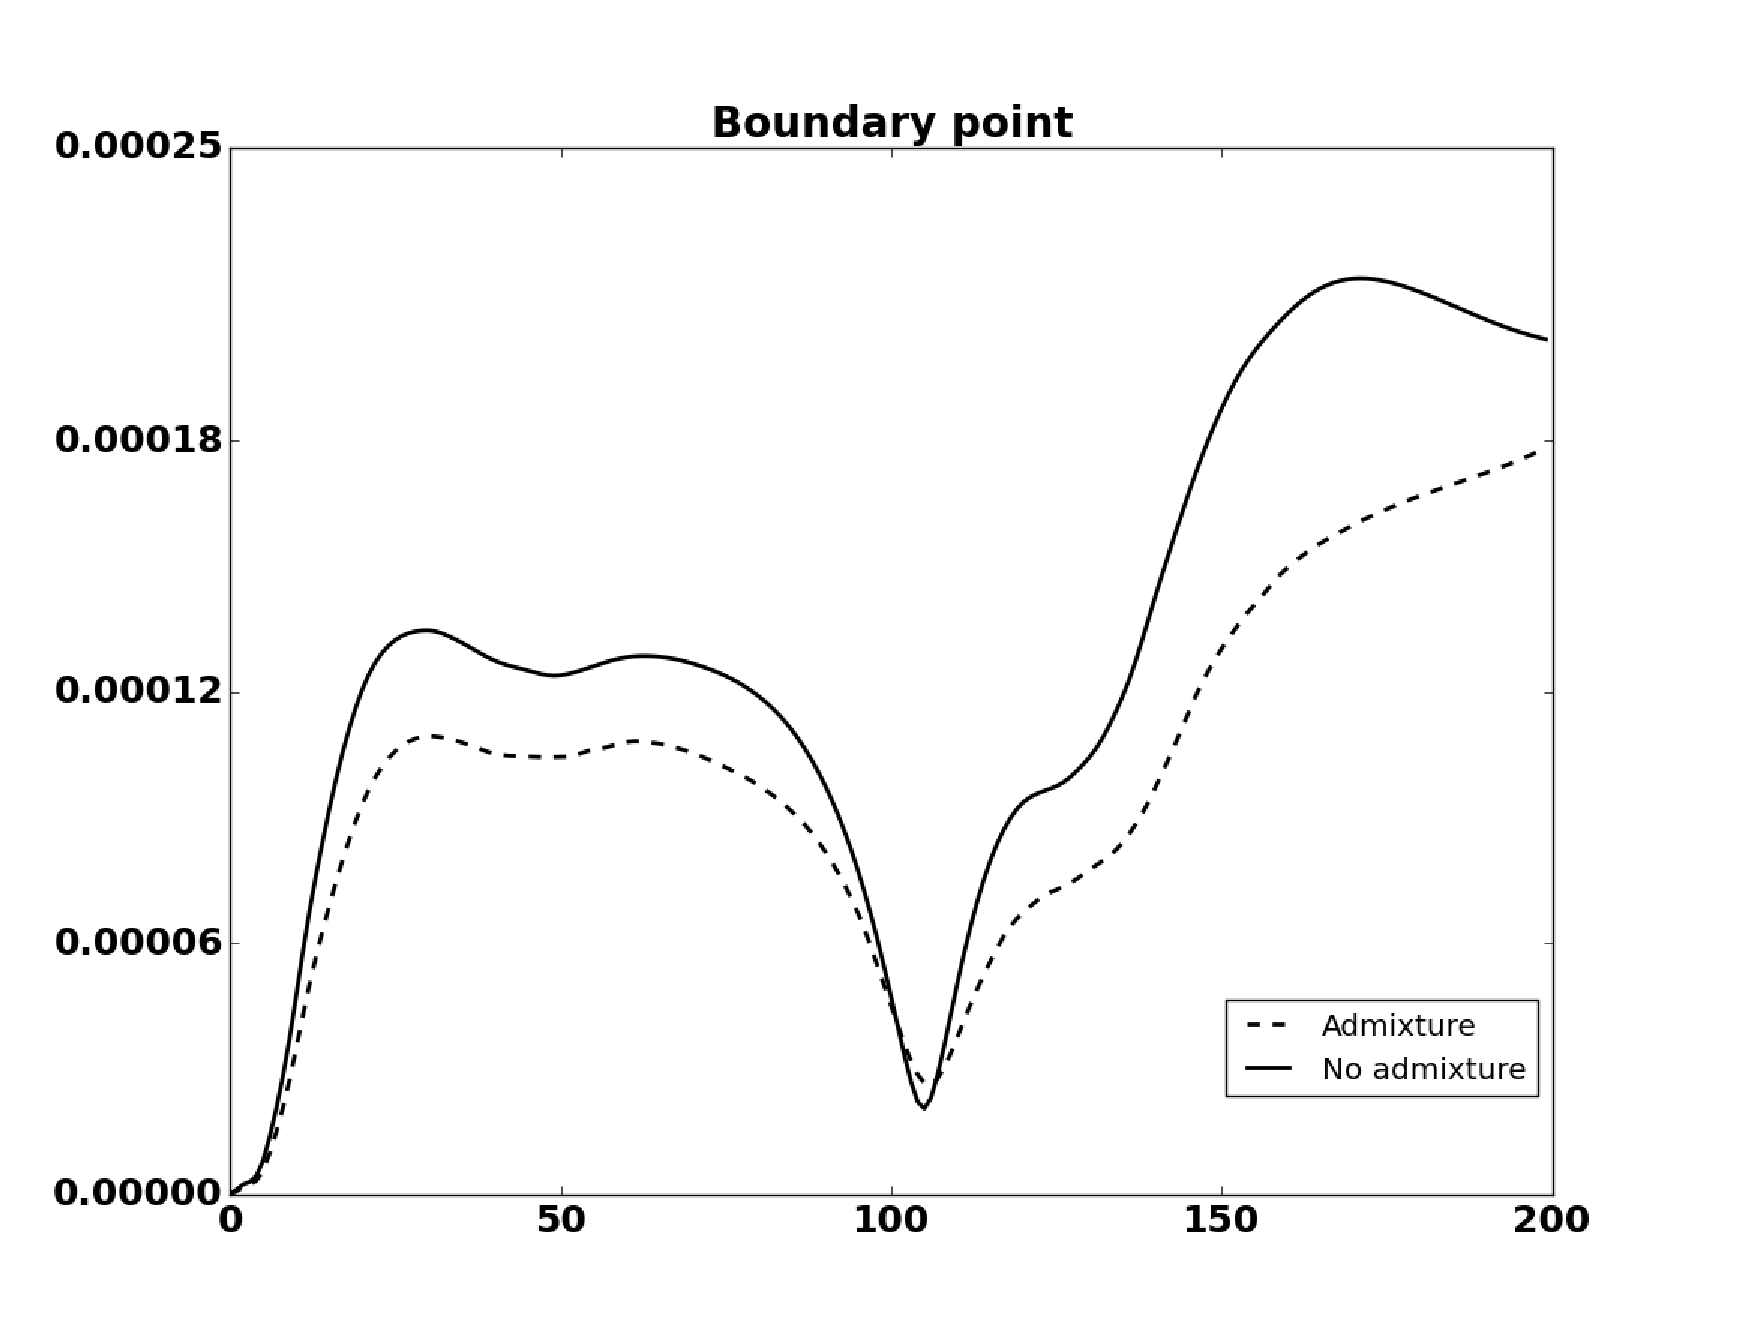
\includegraphics[width=8.5cm]{forces_boundary_point_eng_adaptive_bold.eps}

b

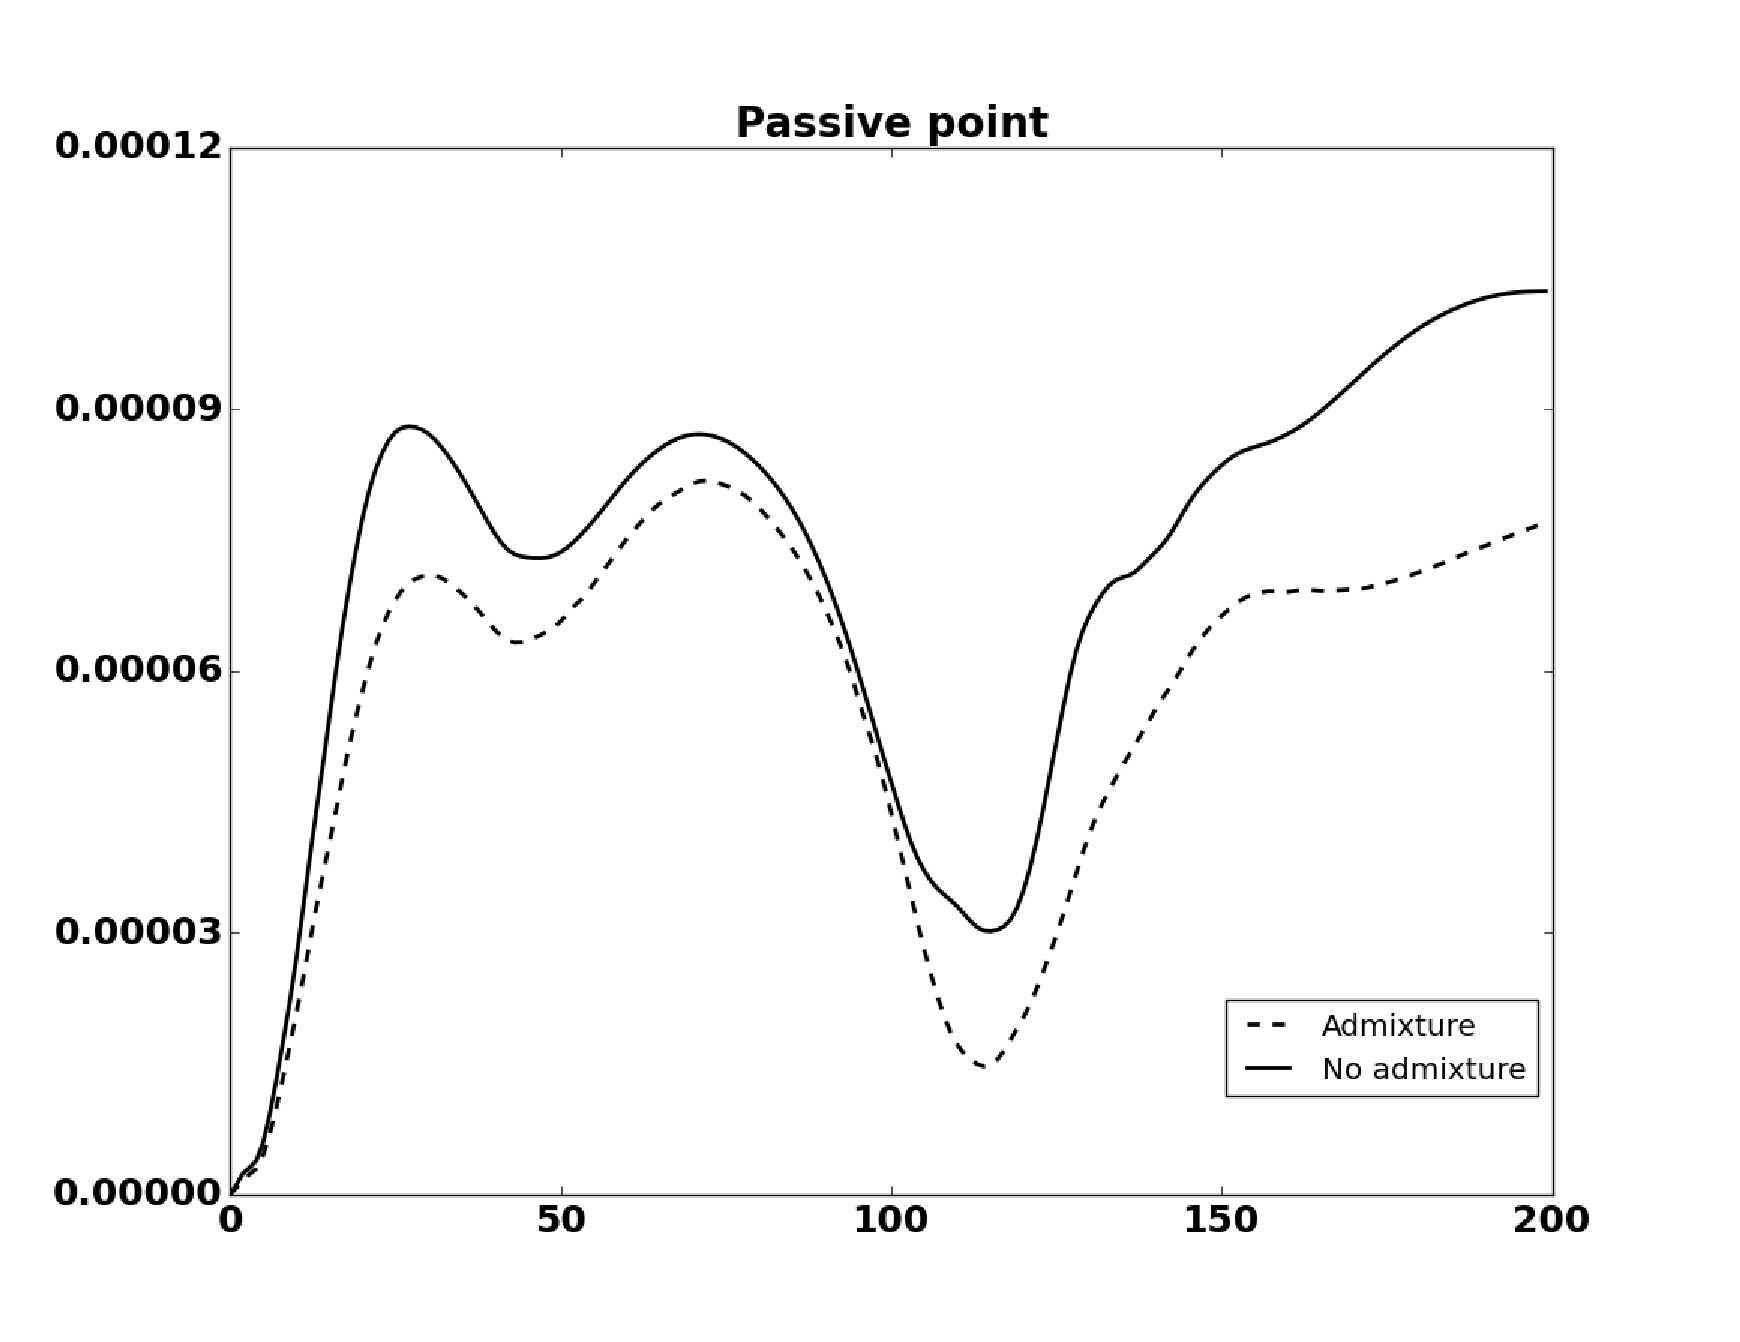
\includegraphics[width=8.5cm]{forces_passive_point_eng_adaptive_bold.eps}

c

\caption{Зависимость напряжения от времени для трех точек на фиброзном кольце
    для случаев без примеси (непрерывная линия) и с примесью (штриховая линия).
    На первом графике (a) изображена зависимость для "Активной точки", на
    втором (b) - для "Точки на границе", на третьем (c) - для "Пассивной
    точки"}
\label{fig:fibrouse_forces}
\end{figure}

Как видно из рис. \ref{fig:fibrouse_forces}, качественно величина
напряжения для каждой точки демонстрирует схожую динамику изменения, но
при этом в области крепления и рядом с осями, если мы рассматриваем однородную жидкость
и постоянную вязкость, возникают б\'{о}льшие напряжения, чем в случае использования модели
течения с переменной плотностью и вязкостью.

\section{Заключение}

Построенная модель работы искусственного сердечного клапана и метод 
её реализации, учитывающая течения крови с переменной плотностью и 
вязкостью, позволяет получать картины движения створок клапана для разных 
геометрий, изменение структуры жидкости при взаимодействии со створками, 
анализировать величину напряжений, возникающие при их движения. 

\funding{Работа проводится в рамках проектной части гос задания 1.630.1.2014/K} %%% Specify the organizations and/or grants if required...

\bibliographystyle{plain}
\begin{thebibliography}{18} %%% The refences should be ordered by the authors
\bibitem{aha2015} Association A.H., {\em Heart disease and stroke statistics} \url{https://www.heart.org/idc/groups/ahamah-public/@wcm/@sop/@smd/documents/downloadable/ucm_470704.pdf}, 2015
\bibitem{duke2015} Institute D.C.R. {\em Adult cardiac surgery database, executive summary} \url{http://www.sts.org/sites/default/files/documents/2015Harvest2_ExecutiveSummary.pdf}, 2015. 
\bibitem{bokeria2008} Бокерия Л.А., Скопин И.И., Сазонов М.А., Тумаев Е.Н., Механическое напряжение в створках митрального клапана и биопротеза в митральной позиции. влияние геометрии фиброзного кольца на величину напряжения створок. {\em Клиническая физиология кровообращения. Научный центр сердечно-сосудистой хирургии им. АН Бакулева РАМН} {\bf 2} (2008), 73--80.
\bibitem{kim2009} Kim H.S. Nonlinear multi-scale anisotropic material and structural models for prosthetic and native aortic heart valves. {\em Georgia Institute of Technology}, 2009.
\bibitem{taylor1998} Taylor C.A., Hughes T.J., Zarins C.K. Finite element modeling of blood flow in arteries. {\em Computer methods in applied mechanics and engineering} {\bf 158} (1998), 155--196.
\bibitem{zhang2004} Zhang Y., Bajaj C. {\em Finite element meshing for cardiac analysis} Univ. of Texas at Austin: ICES Technical Report, 2004
\bibitem{black1991} Black M. et al. A three-dimensional analysis of a bioprosthetic heart valve {\em Journal of Biomechanics} {\bf 24} (1991), 793--801.
\bibitem{peskin2002} Peskin C.S. The immersed boundary method {\em Acta numerica} {\bf 11} (2002), 479--517.
\bibitem{griffith2012} Griffith B.E. Immersed boundary model of aortic heart valve dynamics with physiological driving and loading conditions {\em International Journal for Numerical Methods in Biomedical Engineering} {\bf 28} (2012), 317--345. 
\bibitem{ma2013} Ma X. et al. Image-based fluid--structure interaction model of the human mitral valve {\em Computers \& Fluids} {\bf 71} (2013), 417--425.
\bibitem{gummel2013} Gummel E.E, Milosevic H., Raguling V.V., Zakharov Y.N., Zimin A.I.,  Motion of viscous inhomogeneous incompressible fluid of variable viscosity {\em Zbornik radova konferencije MIT} (2013) 2013--2014.  
\bibitem{dolgov2015vestnik} Долгов Д.А., Захаров Ю.Н. Моделирование движения вязкой неоднородной жидкости в крупных кровеносных сосудах {\em Вестник КемГУ} {\bf 62} (2015), 30--34. 
\bibitem{dolgov2015scp} Dolgov D., Zakharov Y. Mathematical modelling of artificial heart valve performance {\em ''Stability and control processes'' in memory of vI zubov (sCP)} (2015), 518--521.
\bibitem{karo1978} Каро К., {\em Механика кровообращения}. Мир, Москва, 1978.
\bibitem{whitmore1968} Whitmore R.L. {\em Rheology of the circulation}. Pergamon, 1968.
\bibitem{belotserkovsky1984} Белоцерковский О.М. {\em Численное моделирование в механике сплошных сред}. Наука, Москва, 1984.
\bibitem{yanenko1967} Яненко Н.Н. {\em Метод дробных шагов решения многомерных задач математической физики}. '' Наукa'', Новосибирск, 1967.
\bibitem{klyshnikov2013} Клышников К.Ю., Овчаренко Е.А., Мальцев Д.А., Журавлева И.Ю., Сравнительная характеристика гидродинамических показателей биопротезов клапанов сердца Юнилайн и Перикор {\em Клиническая физиология кровообращения} (2013) 45--51.
\end{thebibliography}

\end{document}
